\documentclass[11pt,a4paper,twoside,onecolumn,openany,final,oldfontcommands]{memoir}
\usepackage{sty/FOBOS}  % FOBOS SDN style file
\usepackage[hang,flushmargin]{footmisc}

%%%%%%%%%%%%%%%%%%%%%%%%%%%%%%%%%%%%%%%%%%%%%%%%%%%%%%%%%%%%%%%%%%%%%%%%%
%%%%%%%%%%%%%%%%%%%%%%%%%%%%%%%%%%%%%%%%%%%%%%%%%%%%%%%%%%%%%%%%%%%%%%%%
% Things you need to edit:
%   - Document name, numbering, and date; edit the newcommands below.
%   - Authors list; see authors.tex
%   - The contact information for the corresponding author; see corresponding.tex
%   - Any (additional) tex aliases you would like to include; see aliases.tex
%   - BibTex references are included using ref.bib
%   - Main body of the document
%   - Add a line to the revision history

\newcommand{\doclongname}{Science Requirements Document}
\newcommand{\docshortname}{SRD}

\newcommand{\project}{FOBOS}
\newcommand{\wbs}{TOP}
\newcommand{\doctype}{DOC}
\newcommand{\docnumber}{001}

% Pre-release versions are 0A - ZZ; Release versions should be 01-99
\newcommand{\docversion}{0A}
\newcommand{\docreleaseDate}{2020-09-17}  % Please use ISO-8601 YYYY-MM-DD format.

%%%%%%%%%%%%%%%%%%%%%%%%%%%%%%%%%%%%%%%%%%%%%%%%%%%%%%%%%%%%%%%%%%%%%%%%
%%%%%%%%%%%%%%%%%%%%%%%%%%%%%%%%%%%%%%%%%%%%%%%%%%%%%%%%%%%%%%%%%%%%%%%%

% Document Designation Number
\newcommand{\docsysnum}{{\project}.{\wbs}.{\doctype}.{\docnumber}.V{\docversion}}

%% Set footers to use document info
%% ================================
\makeoddfoot{Ruled}{\docsysnum}{}{\thepage\ / \thelastpage}
\makeevenfoot{Ruled}{\thepage\ / \thelastpage}{}{\docsysnum}

%%% Packages for TESTING
\usepackage{lipsum}
\listfiles

%% ALIASES

%\newcommand{\asic}{Application Specific Integrated Circuit}
%\newcommand{\DRC}{Design Reference Case}
%\newcommand{\keck}{W.~M.~O. Keck Observatory}
%\newcommand{\ie}{\emph{i.e.\ }}
%\newcommand{\scales}{Santa Cruz Array of Lenslets for Exoplanet Spectroscopy}
%\newcommand{\inst}{FOBOS}
%\newcommand{\sidecar}{SIDECAR}
%\newcommand{\SIDECAR}{System for Image Digitization, Enhancement, Control and Retrieval}
%\newcommand{\SWG}{Science Working Group}
%\newcommand{\tis}{Teledyne}
%\newcommand{\TIS}{Teledyne Imaging Sensors}
%\newcommand{\ucscfull}{University of California Santa Cruz}
%\newcommand{\ucsc}{UCSC}
%\newcommand{\wrt}{with respect to}

\newcommand{\farcm}{\mbox{\ensuremath{.\mkern-4mu^\prime}}}  % fractional arcminute: 0.'0
\newcommand{\farcs}{\mbox{\ensuremath{.\!\!^{\prime\prime}}}}  % fractional arcsec: 0.''0
\newcommand{\fdg}{\mbox{\ensuremath{.\!\!^\circ}}}  % fractional degree:  0.¡0
\newcommand{\arcdeg}{\ensuremath{^{\circ}}}  % degree symbol:  ¡
\newcommand{\arcmin}{\ensuremath{^{\prime}}}  % degree symbol:  ¡
\newcommand{\arcsec}{\ensuremath{^{\prime\prime}}}  % degree symbol:  ¡
\newcommand{\sun}{\ensuremath{\odot}}  % sun symbol

\newcommand{\msun}{M$_{\odot}$}
\newcommand{\Msun}{{\rm M}_{\odot}}
\newcommand{\Hz}{{\rm Hz}}
\newcommand{\erg}{{\rm erg}}
\newcommand{\yr}{{\rm yr}}
\newcommand{\cm}{{\rm cm}}
\newcommand{\kms}{{\rm km s$^{-1}$}}
\newcommand{\s}{{\rm s}}
\newcommand{\Mpc}{{\rm Mpc}}
\newcommand{\Halpha}{{H$\alpha$}}
\newcommand{\Hbeta}{{H$\beta$}}
%\newcommand{\Mgb}{{Mg$_{\rm b}$}}
\newcommand{\Mgb}{Mg{\it b}}
\newcommand{\Reff}{{R$_{e}$}}
\newcommand{\HI}{{\sc H\,i}}
\newcommand{\HII}{{\sc H\,ii}}
\newcommand{\photoz}{photo-$z$}

\newcommand{\gaia}{\textit{Gaia}}
\newcommand{\euclid}{\textit{Euclid}}



\definecolor{lblue}{rgb}{0.48,0.65,0.7}
\def\DanM#1{\noindent{\textcolor{lblue}{\textbf[$\spadesuit$ #1]}}}
\def\YST#1{\noindent{\textcolor{lblue}{\textbf[YST: #1]}}}
\def\NS#1{\noindent{\textcolor{lblue}{\textbf[NS: #1]}}}

%%%% BEGIN DOCUMENT
\begin{document}
\bibliographystyle{sty/aasjournal}

%%% FRONTMATTER
\frontmatter
{\begingroup
\newlength{\drop}
\drop=0.1\textheight
\begin{flushleft}
    
\includegraphics[width=\textwidth]{figs/logo/FOBOS_LOGO_FINAL.png}

    \vspace{0.5\drop}
    \begin{Spacing}{1.5}
    {\huge \doclongname\\ (\docshortname)}
    \end{Spacing}
    \vfill

    \vfill
    {\Large
    % Authors
Kyle B.\ Westfall,\textsuperscript{1}
Kevin A.\ Bundy,\textsuperscript{1,2}
Daniel C.\ Masters,\textsuperscript{3}
Joseph N.\ Burchett,\textsuperscript{2}
V.\ Ashley Villar,\textsuperscript{4}
R.\ Michael Rich,\textsuperscript{5}
Benjamin F.\ Williams,\textsuperscript{6}
Nathan Sandford,\textsuperscript{7}
and
Yuan-Sen Ting \textsuperscript{8}

% Affiliations
\begin{small}
\textsuperscript{1}University of California Observatories;
\textsuperscript{2}University of California, Santa Cruz;
\textsuperscript{3}IPAC, California Institute of Technology;
\textsuperscript{4}Columbia University;
\textsuperscript{5}University of California, Los Angeles;
\textsuperscript{6}University of Washington;
\textsuperscript{7}University of California, Berkeley
\textsuperscript{8}The Australian National University
\end{small}


    }
    \vfill

    {\LARGE \bfseries \docsysnum} \\
    \docreleaseDate{} \\
    \thelastpage\ pages

\end{flushleft}
\vspace*{0.5\drop}
\endgroup}

\thispagestyle{empty}  % Title page has no page number shown.

\clearpage
\setupmaintoc
\tableofcontents 

\clearpage
\listoffigures

\clearpage
\listoftables

%: PREFACE
\chapter{Corresponding Author}
%
\begin{table}[htp]
\begin{center}
\begin{tabular}{l}
    Kyle B.\ Westfall, \emph{FOBOS Project Scientist} \\
    University of California Observatories \\
    University of California, Santa Cruz \\
    1156 High Street\\
    Santa Cruz, CA 95064 USA \\
    \\
    +1-831-459-4362 \\ 
    \\
    {\ttfamily westfall@ucolick.org}
\end{tabular}
\end{center}
\end{table}%



%%%%%%%%%%%%%%%%%%%%%%%%%%%%%%%%%%%%%%%%%%%%%%%%%%%%%%%%%%%%%%%%%%%%%%%%
%%%%%%%%%%%%%%%%%%%%%%%%%%%%%%%%%%%%%%%%%%%%%%%%%%%%%%%%%%%%%%%%%%%%%%%%
% The rest of the document editing begins here

%-----------------------------------------------------------------------
% Executive Summary
\chapter{Executive Summary}

\edit{This is the FOBOS science-requirements document.}

%-----------------------------------------------------------------------


%-----------------------------------------------------------------------
% Main document body
\mainmatter

\chapter{Introduction}

Led by the Vera C.~Rubin Observatory Legacy Survey of Space and Time (LSST)\footnote{For the first ten years of operation, Vera C.~Rubin Observatory will perform the Rubin Observatory Legacy Survey of Space and Time (LSST). The National Science Foundation (NSF) and the US Department of Energy (DOE) are joint partners in the Rubin Observatory Project and Operations.} and NASA-supported missions like \euclid\footnote{\euclid\ is led by the European Space Agency with significant NASA involvement and will launch in 2022. Its primary mission is a 15,000 deg$^2$ imaging and grism survey in optical and near-IR wavebands.} and the Nancy Grace Roman Space Telescope,\footnote{Previously referred to as the Wide-Field Infrared Survey Telescope (WFIRST), the Nancy Grace Roman Space Telescope is expected to launch in the mid 2020's.} astronomy is entering a new era of unprecedented deep-imaging campaigns that will survey huge volumes of the universe. From the emergence of the earliest galaxies from a baryonic ``primordial soup,'' through the epoch of cosmic expansion, to the evolved structure of present-day galaxies in our own Local Group and the promise of time-domain discoveries, images from these surveys will provide unprecedented insights into key epochs of cosmic history. As such, these surveys were ranked as top priorities in the Astro2010 decadal survey, resulting in a significant investment of U.S.\ funding agencies in their success.

The need for spectroscopic follow-up of these vast imaging campaigns is obvious.  Indeed, the success of the Sloan Digital Sky Survey (SDSS) and anticipated for the Dark Energy Spectroscopic Instrument (DESI) has made clear the scientific value of coupling panoramic imaging with intensive spectroscopic follow-up, both in terms of new discoveries and in dramatically improving our statistical understanding of the cosmos.  However, at the end of the next decade, these facilities will deliver photometric data across vast areas 1,000 times deeper than SDSS imaging, and \textit{no current U.S.~facility is capable of obtaining spectroscopic follow-up at these depths} at the level required to capitalize on the $\approx$\$4B U.S.\ investment in these projects. In fact, an SDSS-like spectroscopic study of 1 million galaxies at LSST depths would require 300 years of observing on the largest telescopes with current instrumentation!

It has long been recognized that a new spectroscopic facility is needed to meet the challenge presented by this era of deep, panchromatic imaging. For example, the National Research Council's 2015 report, ``Optimizing the U.S. Ground-Based Optical and Infrared Astronomy System'' \citep{NAP21722} states:
%
\noindent\begin{center}\mbox{\parbox{0.95\linewidth}{
%
The National Science Foundation should support the development of a wide-field, highly multiplexed spectroscopic capability on a medium- or large-aperture telescope in the Southern Hemisphere to enable a wide variety of science, including follow-up spectroscopy of Large Synoptic Survey Telescope\footnote{Now renamed to be the Rubin Observatory Legacy Survey of Space and Time.} targets. Examples of enabled science are studies of cosmology, galaxy evolution, quasars, and the Milky Way.
%
}}\end{center}
%
Additionally, workshops organized by the National Optical Astronomy Observatory\footnote{NOAO recently joined with Gemini Observatory and Rubin operations to create NSF's National Optical-Infrared Astronomy Research Laboratory (NOIRLab).} in 2013 and 2016, the latter at request of the NSF, reported specific spectroscopic needs for follow-up of LSST sources in all science areas.  In particular, the 2016 report notes that a critical resource in need of prompt development is to ``Develop or obtain access to a highly multiplexed, wide-field optical multi-object spectroscopic capability on an 8m-class telescope.''

Particularly for the U.~S.\ astronomical community, the twin 10m telescopes of the W.~M.~Keck Observatory (WMKO) represent a compelling avenue to meet this need:  More than 60\% of the LSST footprint and three of its deep-drilling fields (COSMOS, XMM-LSS, and E-CDFS) are within the WMKO visibility window.  Compared to other ongoing efforts to meet upcoming spectroscopic needs \citep{mega2019, mse2019, spectel2019}, WMKO provides an \textit{existing} telescope infrastructure with a 10-m aperture, and, given its site and mirror coatings, is uniquely sensitive toward the atmospheric limit in the UV.  The limited multiplex capacity and sensitivity (compared to more modern equivalents) of its current instruments for optical spectroscopy motivates the need for a much more capable instrument.  Moreover, it is significantly more cost effective to invest in a new instrument for an existing facility than it would be to build an entirely new 10m-telescope$+$spectroscopic facility in the southern hemisphere.

Supporting spectroscopic follow-up of large-scale survey missions is already in lockstep with WMKO's strategic goals.  Specifically, the 2016 WMKO Scientific Strategic Plan (SSP) highlights that WMKO ``works best by undertaking sensitive observations of sources found by surveys or other facilities.''  In fact, the 2016 WMKO Scientific Strategic Plan recommended pursuit of ``highly multiplexed, highly sensitive spectroscopy'' as its top-priority design study.  Although largely cast as upgrades to existing instruments (e.g., adding a second DEIMOS channel), Appendix II of the SSP specifically notes recent improvements in the sophistication of fiber-based instruments that are ``improving throughput, increasing sky-subtraction accuracy, and increasing the density of fibers that can be stacked along the fiber pseudo-slit. All of these trends deepen the limiting magnitude attainable with fibers, as well as the number of objects than can be surveyed.''

These considerations have lead to our concept for the \textbf{Fiber-Optic Broadband Optical Spectrograph, FOBOS,} timed to deploy on WMKO's Keck II Telescope in 2028, just as various panoramic deep-imaging surveys begin reaching their target depths.  FOBOS emphasizes flexible and quickly configurable focal-plane sampling with high multiplex, UV sensitivity, and a stable spectral format that supports ultra-deep integrations of $\gtrsim$50 hours, thereby building from and expanding on traditional strengths of WMKO observations.

\section{Derivation of ``Requirements'' in this Document}

As a facility-class instrument, FOBOS will be used to pursue a wide range of scientific goals.  The purpose of this document is to encapsulate the breadth and depth of these goals in a way that flows down to the instrument-defining technical requirements.  This document enumerates and provides the justification for all high-level instrument requirements.  These are further developed at deeper levels of detail in associated design documents for each subsystem.

During its Conceptual Design Phase (CoDP), FOBOS science requirements have been developed by defining a set of \textbf{Design-Reference Programs} (Chapter \ref{chap:key}) that capture the core science that FOBOS \textit{must} enable.  The FOBOS Science Team has developed these programs with the view that they represent the most compelling FOBOS science within its first 5 years on-sky.  These programs are for reference only.  A competitive proposal process will determine the final makeup of approved, large-scale programs ahead of FOBOS commissioning. 

% \edit{section now removed, need to edit this} (2) \textbf{Additional Science Drivers} (Chapter \ref{chap:addsd}) are presented that have not (yet) led to large-scale observing programs, but also represent compelling science that FOBOS \textit{must} enable.

While we developed the Design-Reference Programs and associated requirements in order to explore the full range of required FOBOS capabilities, we constrained this exercise with a set of baseline assumptions.  FOBOS should:

\medskip
\begin{asparaenum}
\item Dramatically improve on the current DEIMOS multiplex of $\sim$100 targets,
\item Adopt a fiber-fed, modular spectrograph design (in order to do so),
\item Provide both single-aperture and integral-field capabilities,
\item Cover the near-UV to 1 $\mu$m wavelength range, and
\item Provide a spectral resolution of $R\sim 3000-5000$.
\end{asparaenum}
\medskip

\noindent It goes without saying that FOBOS should enable transformational science at a minimal total cost that is competitive with other modern instruments of a similar scale. With this context, we define four types of requirements in this document.  At the highest level:

\begin{itemize}
\item \textbf{Program Requirements (P)} define the final measurement fidelity, derived after all observations, that is required to make a given Key Program successful. For example, ``To measure a change in the slope of the initial mass function (IMF) of $X$ dex per ${\rm d}(\log\mathcal{M}_\ast)$ or larger, the equivalent width of the Wing-Ford band must be measured to better than $Y$ dex for $N$ galaxies evenly distributed over a mass range of $\mathcal{M}_1 < \mathcal{M}_\ast < \mathcal{M}_2$.''  

\item \textbf{Science Requirements (S)} define the \emph{instantaneous} ability of FOBOS to obtain observations that satisfy a program requirement.  For example, ``The spectral range must include the Wing-Ford band (989 nm $< \lambda <$ 995 nm) for galaxies at $z \lesssim 0.1$.''  
\end{itemize}

\noindent Program Requirements (P) can flow to both Science Requirements (S) and Instrument (R) or Data (D) requirements.  Science Requirements (S) also flow to Instrument and Data Requirements, but Science Requirements do not flow to Program Requirements.  

\noindent Instrument and Data Requirements translate science goals into technical specifications:

% A useful distinction is that program requirements can flow down to one or more science requirements, but not vice versa. Program and science requirements are signified by \textbf{P} (e.g., \ref{prog:photoz:sample}) and \textbf{S}, respectively.

\begin{itemize}
\item \textbf{Instrument Requirements (R)} define technical capabilities, for example, ``The red spectral limit must be $\geq$ 1.1 $\mu$m.'' 

\item \textbf{Data Requirements (D)} place requirements on software systems that manage the reduction, processing, and storage of data, the data-management systems (DMS), e.g., ``Across program fields observed over many nights, the reduction pipeline shall not introduce scatter greater than 10\% of Poisson compared to a single-visit manual reduction.'' 
\end{itemize}


% This document consolidates the program and science requirements into a series of \textbf{instrument requirements} and \textbf{data requirements}.  Here, we distinguish between requirements that are primarily driven by the instrument hardware from those primarily driven by the software related to the data-management systems (DMS; Chapter \ref{chap:DMS}).  Following from the example above, a relevant instrument requirement would be: ``The red spectral limit must be $\geq$ 1.1 $\mu$m.''  A relevant data requirement would be: ``Systematic errors in the equivalent width of the Wing-Ford band introduced by sky subtraction and flux calibration must not be larger than 10\% of the Poisson error due to photon shot noise.''  

% \noindent Importantly, there is an obvious interplay between the hardware and software requirements that will evolve as the limitations of each are explored. Instrument and data requirements are signified by an \textbf{R} and \textbf{D}, respectively.

In this SRD version, Data Requirements do not differentiate between requirements for the data-\textit{reduction} pipeline (the DMS \textit{Accountant}) versus the data-\textit{analysis} pipeline (the DMS \textit{Alchemist}).  In general, while FOBOS aims to deliver high-level data products for \textit{all} FOBOS data, the FOBOS software systems requirements will be driven by the Design-Reference Programs.

Summary tables provide a mapping from each instrument/data requirement to all associated program/science requirements (Table \edit{x}) and vice versa (Table \edit{y}); each program/science requirement must lead to at least one instrument/data requirement.

\section{Guiding Principles and Assumptions}

In discussing the science requirements, we distinguish between measurement ``precision'' and ``accuracy''. All of our quantitative requirements focus on measurement precision, which includes only uncertainty propagated from raw measurement uncertainties under a specific set of model assumptions. Assessments of the \textit{accuracy} of a given measurement are generally a model-dependent assessment and, therefore, beyond the scope of this document.

\section{Document Outline}

The Science Requirements Document is organized as follows:  Each of the Design-Reference Programs are motivated and presented in Chapter \ref{chap:key}.  The chapter is organized into one section per primary science program goal.  Many programs share a common discipline, and multiple programs are more efficiently executed simultaneously.  We close Chapter \ref{chap:key} by discussing possible observational synergies between programs. 

% TODO: We need a chapter devoted to machine-learning applications.

In Chapter \ref{chap:instr}, we first consolidate the program and science requirements from Chapter \ref{chap:key} into a few high-level technical requirements for, e.g., spatial sampling (Section \ref{sec:sampling}) and spectrophotometry (\ref{sec:spectrophotometry}). The Chapter ends with a section that provides the consolidated tables with instrument requirements pointing to their motivating program and science requirements. Chapter \ref{chap:DMS} mirrors Chapter \ref{chap:instr} but focuses on the data requirements and a discussion of the data management systems needed to meet these requirements.

% TODO: Move documentation chapter content to the PEP 
% Finally, Chapter \ref{chap:doc} discusses the documentation plans for FOBOS development.

\newpage

\chapter{Design-Reference Programs}
\label{chap:key}

% Requirement redundancy in the science programs
%   - weigh this against overwhelming the reader

FOBOS is a facility-class instrument at Keck, emphasizing flexible and quickly configurable focal-plane sampling, UV sensitivity, and a stable spectral format that supports ultra-deep integrations of $\gtrsim$50 hours.  Multiple observing modes will be possible, including PI-led programs, survey-level campaigns, and queue-scheduled observations.  In combination, these modes will enhance overall science return by enabling human interaction/intervention while maximizing efficiency.  

While designed to support a broad range of science applications, the FOBOS concept is driven by a series of ``Design-Reference'' Programs centered on studies of the nature of Dark Energy and Dark Matter, the formation of galaxies, the physical properties of kilonovae and other well-localized transients, and the assembly history of the Andromeda Galaxy and its environment.  Each program would advance the scientific frontier anticipated at the time of FOBOS commissioning, both in terms of direct interpretation of the observations themselves and their use in machine-learning methods that can train and deliver physical inferences for the upcoming trove of photometric samples.  This chapter presents the scientific motivation, execution details, program requirements, and success metrics for each program.

\noindent \textbf{Allocated Program Observing Time.}  To set requirements on capabilities like multiplex and sensitivity, we must often require that design-reference programs be completed with a given allocation of observing time, specified here as clear-weather nights (no weather factor) unless otherwise specified.  Following the history of past large-program campaigns at WMKO, we adopt a maximum program allocation of 130 nights over 5 years (about 15\% of total available dark time).  A five-year timescale is common among astronomical surveys and reflects the speed of scientific progress in the field and the timescales of graduate students and postdocs.  Keck is highly over-subscribed, with a large and diverse user pool carrying out an array of PI-led programs, so if they have any hope of being realized, most of the design-reference programs below should complete in \emph{far less} than 130 nights, with 5-10 nights anticipated per-year over a 5-year timespan.  

% To illustrate FOBOS's scientific potential, we present the science drivers and observing strategies for these design-reference programs.  Table \ref{tab:progreq} summarizes the details of each program and illustrates FOBOS's ability to interleave multiple programs with disparate scientific goals (\S \ref{sec:addsci}).  The final definition of FOBOS's design-reference programs, including detailed sample designs, scientific deliverables, and time requests, will be developed in the next phase through a community-wide competition organized jointly with NSF's NOIRLab and WMKO.

\section{Dark Energy: Photometric Redshift Training}
\label{sec:photozs}

Stage-IV cosmology missions --- like the Vera C.~Rubin Observatory Legacy Survey of Space and Time (LSST), the ESA/NASA \euclid\ mission, and the NASA-led Nancy Grace Roman Space Telescope (Roman) --- will obtain multi-band imaging data with unprecedented depth and survey area in the coming decades.  Current survey baselines for LSST will provide \textit{ugrizy} optical imaging of $\sim$18,000~deg$^{2}$ with a detection limit 1,000 times fainter than the Sloan Digital Sky Survey (SDSS), complemented by deep near-IR imaging by Roman for an overlapping $\sim$2000~deg$^{2}$.  Measurements drawn from these data of galaxy positions and gravitational shear as a function of distance over vast cosmic volumes will be used to delineate cosmic expansion and the growth of large-scale structure. Critically, the distances used for these measurements must be estimated by photometric redshifts (photo-$z$s), given the infeasibility of obtaining spectroscopic redshifts (spec-$z$s) for the expected magnitude distribution of the billions of sources imaged by these surveys (see Figure \ref{fig:cosmos_magdist}).  This reliance on photo-$z$s has led to significant effort devoted to understanding their influence on the derived cosmological parameters \citep{huterer06, hearin10, newman15, LSSTDESCSRD}.  The consensus of these studies is that improving galaxy photo-$z$ estimates represents one of the most significant gains to be made in the precision of the cosmological parameters.

Limiting uncertainties in photo-$z$ estimates involves improving photo-$z$ \textbf{training} and \textbf{calibration} \citep{newman15}.  Training focuses on improving photo-$z$s by, e.g., ensuring that the underlying spectroscopic redshifts used to establish the relationship between galaxy color and redshift sample the relevant parameter space \citep{masters15, hemmati18}.  Photo-$z$ calibration involves quantification of the accuracy and precision with which photo-$z$s map to spec-$z$s for \textit{all} galaxies used to measure dark-energy parameters of interest.  Both pursuits are critical to improving the constraining power of and minimizing the biases in the resulting cosmological parameters \citep{LSSTDESCSRD}.

The specific needs for photo-$z$ training and calibration for Dark Energy have been laid out in series of Astro2020 white papers that detail required obseerving programs and advocate for new instruments like FOBOS \citep{newman19, hlovek19, mandelbaum19}.  In particular, \citet{newman15, newman19} outline an observing program that improves photo-$z$ training via spectroscopy of thousands of galaxies at very faint magnitudes ($i_{\rm AB} \lesssim 25.3$).  The combination of sample size and magnitude distribution is nearly impossible to achieve with current instrumentation.  \citep{masters19}, meanwhile, describe the significant efforts underway to obtain Keck spectroscopy in service of \euclid\ photo-$z$ training.  More ambitious programs will be needed for fainter LSST/Roman samples.


% LSST will provide a crucial extragalactic dataset in the late 2020s, providing deep \textit{ugrizy} optical imaging of $\sim$18,000~deg$^{2}$, while WFIRST will obtain deep near-IR imaging for $\sim$2000~deg$^{2}$, overlapping the LSST footprint. FOBOS will be well-positioned to contribute critical follow-up spectroscopy for both missions, with the ability to efficiently observe sources as far south as $-30^\circ$, comprising $\sim$60\% of the current baseline LSST footprint.

\begin{figure}
\begin{center}
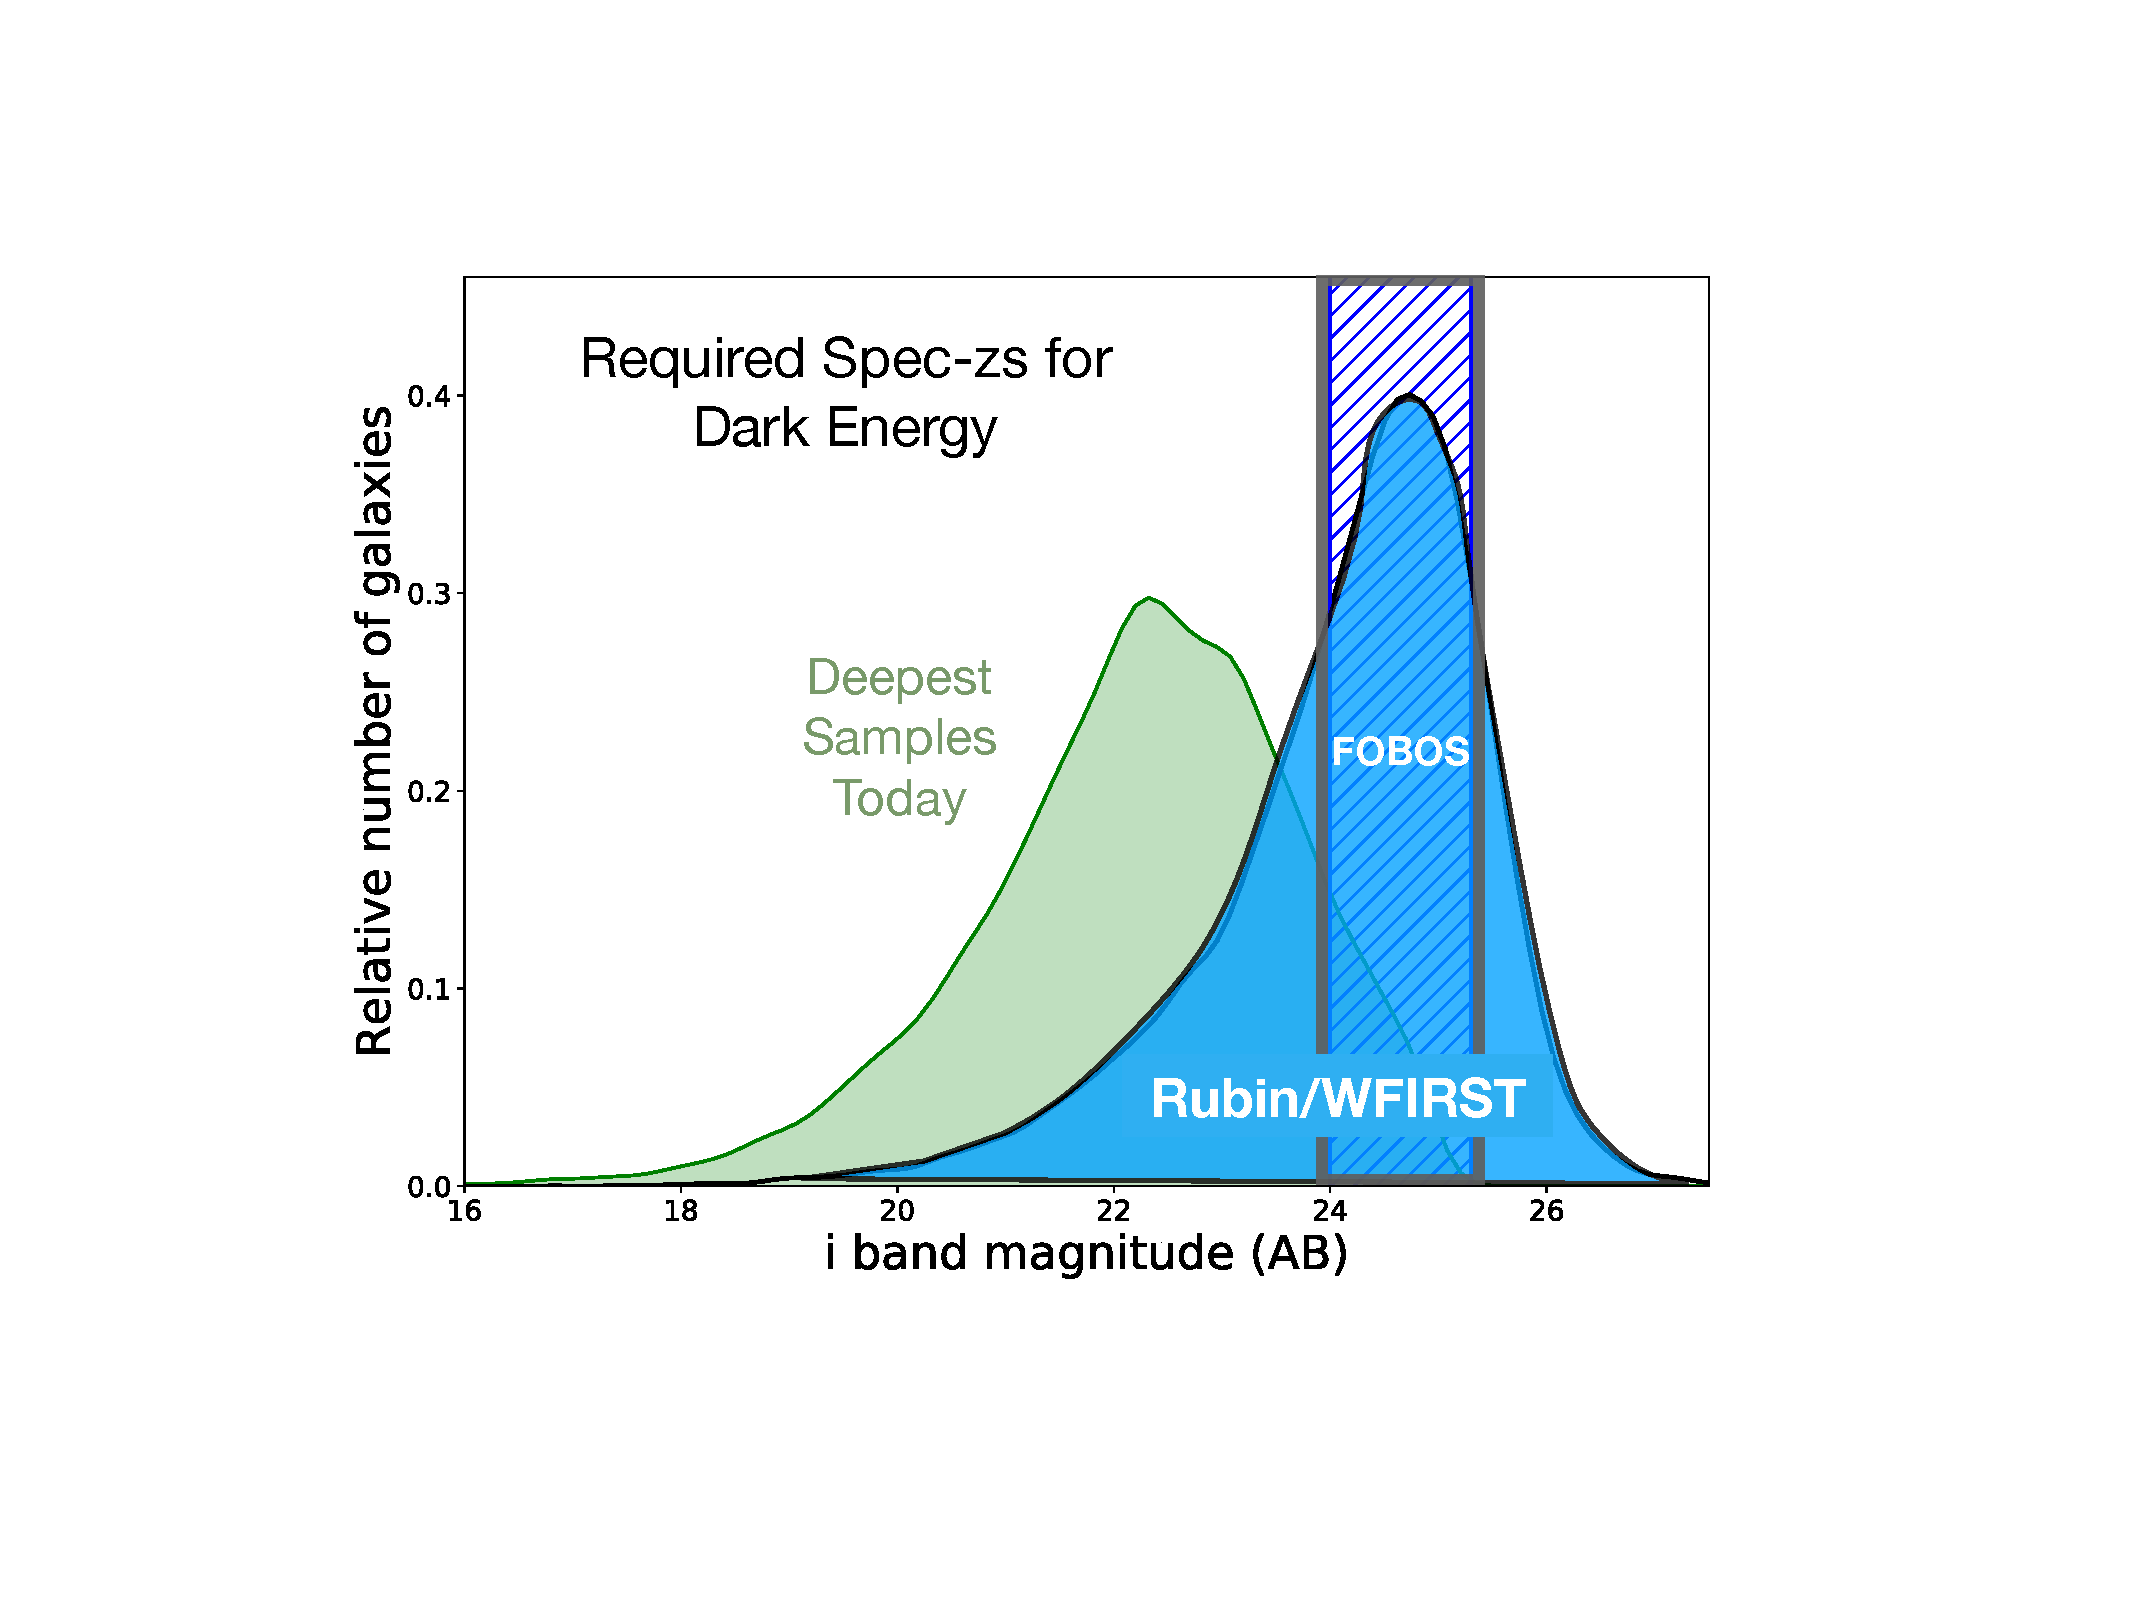
\includegraphics[width=0.7\textwidth]{figs/fobos_cosmology_v2.pdf}
\end{center}
\caption[Magnitude distribution of spec-$z$ samples]{Magnitude distribution of secure spec-$z$ samples in existing deep fields from, e.g., DEEP2, VVDS, VIPERS, C3R2, and zCOSMOS (\textit{green}), compared with the anticipated distribution of the LSST/WFIRST weak-lensing sample derived in \citet[][\textit{blue}]{hemmati18}. Ultra-deep (50hr) exposures in the FOBOS cosmology program are designed to obtain spec-$z$s for $\sim$15k faint galaxies in the hatched region, representing roughly 50\% of the weak-lensing sample of these missions and weakly constrained by current spec-$z$ samples. The FOBOS cosmology program would operate over 12 independent regions to mitigate cosmic variance, employing a careful selection to explore the full color-magnitude parameter space efficiently, as in \cite{masters15}. }
\label{fig:cosmos_magdist}
\end{figure}

FOBOS will provide uniquely powerful spectroscopy capabilities for photo-$z$ training, until at least the second generation of instruments on ELTs (E-ELT, TMT, GMT).  It will excel for sources with spectral features too blue or fluxes too faint for other instruments, like PFS,\footnote{Subaru's Prime Focus Spectrograph (PFS) commissioning in 2022.} but that dominate by number (Fig.~\ref{fig:cosmos_magdist}).  For example, Rubin Observatory will begin reaching the LSST target 5$\sigma$ point-source depth of $i_{\rm AB} = 26.8$ in 2029.   FOBOS spectroscopic follow-up to $i_{AB} = 25.3$ for extended sources will provide a well-matched training sample\footnote{\citet{newman15} emphasize that photo-$z$ ``calibration'' can be accomplished by cross-referencing all-sky surveys of various low-density tracers like quasars and associated absorbers, luminous red galaxies, and emission-line galaxies.} that will \textit{increase LSST's dark energy figure-of-merit by 20--40\%} \citep{newman15}. 

 Additionally, because FOBOS has no ``redshift desert'' (its blue wavelength coverage allows redshift determination at $1.5\lesssim z \lesssim2.5$ via Ly$\alpha$ or nearby UV absorption features), FOBOS observations will reduce the need for expensive, space-based\footnote{Ground-based near-IR spectroscopy is too contaminated by night-sky emission lines to provide spec-$z$s at the required level of completeness \citep{newman15}.} near-IR spectroscopy of galaxies with $z > 1.5$.  

 Beyond enhancing cosmological analyses, the resulting galaxy sample would have a major impact on galaxy-evolution studies by providing the spectroscopic coverage needed to fully leverage photometry for billions of galaxies.  % (see \S\ref{sec:ML}). 

 The FOBOS Dark Energy Program would require 62.5 dark nights over five years.
% \edit{Can Dan M. update this with some of the work he did in the lead-up to the MsRI proposal?  I.e., SOM results and expected "no error" photo-z precision?  Also, add plot from Rachel and Husni?}

\noindent \textbf{FOBOS Dark Energy Program Requirements:}

\begin{programrequirement}
\reqitem Sample size of at least 15,000 high-confidence spectroscopic redshifts in the magnitude range $24 < i_{\rm AB} < 25.3$ to provide maximum statistical precision on the mapping of color-space to redshift-space. \label{prog:photoz:sample}

% , populating the region of the galaxy color/magnitude space relevant to the LSST-\euclid-Roman photometric samples, which is largely unconstrained by existing spectroscopic surveys. 

\reqitem At least 12 independent fields to limit cosmic variance \citep[see][]{newman15}, with field centers that span a large range in right ascension for efficient program scheduling. \label{prog:photoz:fields}

\reqitem Each field must be at least 20\arcmin\ in diameter and contain roughly 1700 viable targets.  This number assumes 15,000 galaxies observed (\ref{prog:photoz:sample}) over the number of independent fields (\ref{prog:photoz:fields}), and it accounts for the expected redshift completeness (75\%; \ref{prog:photoz:zcomplete}).


\reqitem At least 10 fields must also overlap with the LSST footprint and be within the visibility window of Keck II for no less than two consecutive hours.
\reqitem At least one field must be in the NEP for overlap with \euclid\ and (Subaru) Hyper Suprime-Cam observations.
\reqitem At least three of these fields must overlap LSST deep-drilling fields.

\reqitem Objects observed must achieve an $i$-band-weighted signal-to-noise of 2 per angstrom to ensure 75\% redshift completeness. \label{prog:photoz:snperspec}

% KBundy 2021-04-04:  Newman+13 Fig 47 shows 75% redshift success at S/N = 0.75 per DEIMOS 0.33 A pixel (with 1200 line grating).  Multiply by sqrt(3) and S/N per angstrom is 1.3.  But this is for "all" galaxies and r-band, so until we do simulations, let's adopt S/N = 2 per angstrom.

\reqitem No target should require more than 50 hours of integration time under dark, spectrophotometric conditions to maintain observing efficiency.  Given requirement \ref{prog:photoz:snperspec}, this means the continuum S/N per object after one hour of observing must be no less than 0.4 per angstrom at $i$-band.  \label{prog:photoz:snperhr}

\reqitem To efficiently build the sample, the program must be able to reconfigure individual fibers in a field to new targets either as targets acquire sufficient S/N for redshift measurements or targets are found to not meet requirement \ref{prog:photoz:snperhr}.
\end{programrequirement}

\medskip
\begin{sciencerequirement}
\reqitem At least 75\% of FOBOS spectra for galaxies at $z<2.5$ with a continuum S/N of 2 per angstrom must result in accurate spectroscopic redshifts. \label{prog:photoz:zcomplete}
\reqitem For spectra satisfying \ref{prog:photoz:zcomplete}, statistical errors in the spectroscopic redshifts of continuum-only sources must be no larger than $\sigma_z/z \sim 10^{-3}$ \edit{check this}.
\reqitem For spectra satisfying \ref{prog:photoz:zcomplete}, statistical errors in the spectroscopic redshifts of emission-line sources sources must be no large than $\sigma_z/z \sim 10^{-4}$ \edit{check this}.
\end{sciencerequirement}

\edit{still useful to have separate requirements for continuum-only and emission-line sources? recast as having a minimum influence on the photo-z training/calibration? can we get the latter from Dan's tests with the SOM?}


%\begin{sciencerequirement}
%\reqitem Redshift precision of 150 \kms{} or better. Stage IV cosmology experiments need to constrain the mean redshift of shear bins to $\lesssim0.2\%$. Redshift samples used for calibration must achieve at least this level of precision per source, which sets this requirement. 
%%
%\reqitem Redshift success rate of 75\% measured in a magnitude bin of width 0.5 mag up to the magnitude limit.  Explanation...
%%
%\reqitem Magnitude limit of $i_{\rm AB} = 25.3$.  This limit corresponds to the expected depth of LSST lensing samples (REF).
%%
%\reqitem Minimum sample size of 15,000, required for sufficient coverage of the photometric color space and for training statistics (REF).
%%
%\reqitem 10 independent fields of minimum 20\arcmin{} diameter in order to average over systematics in the galaxy population owing to sample variance.
%%
%\reqitem Redshift range of $z = $[0.1, 3.5], spanning the distribution of LSST and WFIRST cosmology samples (REF).
%%
%\end{sciencerequirement}


% This program is designed to observe a set of twelve 0.1 deg$^2$ FOBOS pointings arranged evenly in right ascension and chosen to overlap with the LSST, \euclid, and WFIRST footprints.  At least three pointings would include LSST deep drilling fields (COSMOS, XMM-LSS, and E-CDFS).  The program satisfies the sample size, field variance, and depth requirements in \citet{newman15} by obtaining ultra-deep 50-hour integrations of $\sim$15,000 sources at $24 < i_{AB} < 25.3$, a magnitude range that covers the majority of LSST/WFIRST weak-lensing samples.  While near-Poisson performance with such extreme integration times has been demonstrated with fiber spectrographs \citep[e.g.,][]{gu17,childress17}, our team's investigation of critical design factors that enable such performance (Bundy et al., in prep) has defined FOBOS instrument requirements, including a multi-tier calibration system (\S \ref{sec:calib}).  Accounting for expected sensitivity and stability, our exposure-time calculator estimates a continuum S/N$\sim3.5$ ($i$-band) for the faintest sources at these depths, a level known to be sufficient for $>75$\% redshift success (e.g., \citealp{Newman13}, \citealp{masters19}). 

% With 1200 single fibers (per pointing) from two of FOBOS's three spectrographs assigned to cosmology program targets, parallel observations with IFUs fed to its 3rd spectrograph can leverage the ultra-deep exposures needed for targets in the \textit{FOBOS Galaxy Ecosystem Program} (\S \ref{sec:galaxies}).  Photo-$z$ calibrators targeted by single fibers will efficiently span color-magnitude space \citep{masters15, masters19} with dynamic re-allocation of fibers to new targets as successful redshifts are obtained.  This program would request 12.5 dark nights per year.

% TODO: **Move this somewhere relevant**:
% The source density of 40 arcmin$^{-2}$ far exceeds FOBOS's
% fiber density (6 arcmin$^{-2}$).
  

%----------------------------------------------------------

\section{IGM: Tomographic mapping of the Intergalactic Medium}

The fueling and regulation of galaxy growth during the peak formation epoch ($z \sim2$--3) is critically tied to the turbulent and gas-rich ecosystem in which early galaxies evolve. The James Webb Space Telescope (JWST) and upcoming 30-m class telescopes (ELTs) will marshal powerful infrared observations to study the stars and nebular gas at the heart of these early galaxies. But mapping the large-scale gaseous environments and filamentary networks that fuel and ultimately regulate galaxy evolution at these redshifts requires high multiplex absorption-line tomography and rest-frame UV spectral coverage.

% FOBOS enables an ambitious two-prong approach to characterizing galaxy ecosystems on all scales: a detailed tomographic study of the cosmic web at $z>1.5$ combined with an ultra-deep IFU survey of emission from the circumgalactic medium (CGM) of $\sim$180 galaxies at the peak of cosmic star formation.

\edit{Joe will go back over this with updated info from PFS}
The PFS Strategic Survey Program on Subaru (running 2023--2027) \citep{Nagamine:2020_tomography} will complete an important first step in Ly$\alpha$ tomography of the intergalactic medium (IGM) by making a map of structure at $2.1 < z < 2.6$ over 14 deg$^2$.  This map will be relatively coarse, however, with a sight-line density of 1140 deg$^{-2}$.  Although this provides valuable statistical measures of cosmic-web structures, a detailed study of the interplay between the fueling and feedback mechanisms mediated by these structures requires chemical and kinematic diagnostics that are only possible with higher S/N observations at a more fine-grained spatial resolution that is not well-suited to Subaru-PFS.

% TODO:
%   - Need some examples of how these data would be used.
%   - Describe overlap with cosmology program.

An observing program with FOBOS can meet these needs by building a high-resolution map of the IGM via a dense network of Ly-$\alpha$ absorbers associated with targeted structures at $1.6 < z < 2.5$ \citep[see][]{lee16}.  If the PFS survey is completed and distributed in time, this program should prioritize follow-up targets between $1.6 < z < 2.1$ (not accessible to PFS, but where sources are brighter) in these fields, such as protoclusters and galaxy overdensities.  This higher density yields statistical insight at 1 Mpc separations (the scale of individual massive halos) and the ability to stack sightlines to gain further in S/N so that various heavy-element ion transitions can be studied.  The FOBOS IGM program to acquire these data would require 25 clear, dark nights would need to meet the following requirements:


\noindent \textbf{FOBOS IGM Program Requirements:}

\begin{programrequirement}
\reqitem The total area shall be greater than 6 deg$^2$ to survey sufficient volume for detection of rare, proto-cluster structures which will evolve into $z=0$ halos with 10$^{14}$ \msun{}.  This total area will be divided into 12 sub-fields for ease of scheduling.  Each sub-field shall be at least $\sim$0.5 deg$^2$ in order to span the largest structures \citep[see][]{lee16}.

\reqitem For sufficient spatial resolution of the reconstructed IGM tomography (\ref{prog:igm:dens}), each field should include $\sim$5000 targets between $1.6 < z < 2.5$. 
\reqitem Each field should also contain $\sim$3000 galaxies embedded in the cosmic web for comparison of the intergalactic and interstellar media.

\reqitem To detect a minimum \ion{H}{1} column density of $10^{13}$ \edit{check this} with a statistical error of no more than 0.1 dex (25\%)\edit{check this}, 3-hour integrations must reach a ${\rm S/N} \sim 3.5$ at $r_{\rm AB} \approx 24.6$ \edit{check this against ETC}. 

\end{programrequirement}

\medskip
\begin{sciencerequirement}
\reqitem The FOBOS single-aperture sampling density shall deliver efficient ($>70$\% completeness), single-visit target allocation for on-sky source densities of $>$4 arcmin$^{-2}$.  This is commensurate with scales of massive halos; i.e., $\sim$1 Mpc for the most massive galaxy clusters at $z\sim 2$. \label{prog:igm:dens}

% K. Bundy (2021-04-05): The 4 per arcmin^2 comes from 5000 sight-lines plus 3000 embedded galaxies per 0.5 deg^2.  The 70\% is a WAG.

\reqitem FOBOS shall be able to detect Ly$\alpha$ (1216 \AA{}) at a redshift of $z=1.6$.  

\end{sciencerequirement}

%{Baseline source density goals for PFS: 1600/deg$^2$ over 15 deg$^2$.  This sightline density translates to 100 sources over the FOBOS FOV.  From the luminosity function of LBGs, going to a depth of R = 24.5 affords 400 possible $z=2.0-3.0$ sources within a single FOBOS pointing.  A 3-hr observation delivers S/N$\sim4$ per pixel in the g band.  Going to R = 24.6 means 1000 possible sources per FOV at S/N$\sim3.5$.  If we improve on source density over PFS by a factor of 4, we reduce the average sightline separation to $\sim1$ per comoving Mpc, or resolving scales of most massive individual halos!  This leaves 1400 fibers for `embedded' galaxies in the foreground. }

% \note{Joe/Dan/Kyle: play-out the combination of the 2nd program above and the Cosmology program as a practical illustration of what a series of observing nights devoted to these programs might look like. }


\section{CGM: Chemistry and Dynamics of the Circumgalactic Medium at $z\sim2$}

High- and intermediate-ionization transitions, such as \ion{O}{6} ($\lambda_{\rm rest} = 1032, 1037$ \AA) and \ion{C}{4} ($\lambda_{\rm rest} = 1548, 1550$ \AA), probe $10^{5-6}$ K and $10^4$ K gas, respectively.  This temperature range marks the peak in gas cooling and therefore constrains how gas rains onto galaxies to fuel star-formation, as well as tracks feedback processes that establish and regulate the circumgalactic medium (CGM).  Observations of this gas has largely hinged on detection via \textit{absorption} measurements against a background source \edit{refs}.  The ability of these observations to probe the chemodynamical state of the CGM is therefore limited by the number of viable targets through each halo, and stacking of sightlines through many halos is generally required to provide a statistical view of their properties.  If the CGM is instead observed in \textit{emission}, each galaxy halo can be studied individually.

Current Keck instrumentation, namely KCWI, enables the mapping of Ly$\alpha$ emission for individual galaxy halos at $z\sim2$, and metal-line emission has already been studied in some extreme objects. However, significant progress in the field requires deeper observations of a significant sample ($\sim$100 objects) of relatively ``normal'' galaxies (Fig.~\ref{fig:cgmsample}).  Such a sample allows us to explore correlations between host-galaxy and local CGM properties that will provide key observational constraints of cosmological hydrodynamical simulations \edit{refs}.


\noindent \textbf{FOBOS CGM Program Requirements:}

\begin{programrequirement}
\reqitem Spatially-resolved spectroscopy for least 100 individual galaxy halos over a range of host mass and SFR, selecting from Milky-Way-like progenitor galaxies to the most massive brightest-cluster-galaxies today: $9.7 <$ log ($M_*/M_\odot$) $< 11.5$ and spanning quiescent to SFR $\sim 1000$ yr$^{-1}$ \edit{need ref for upper mass limit; Patel+2013a}. \label{prog:cgm:sample}

\reqitem Sufficient S/N to detect and characterize emission line flux at a minimum level of \edit{XX} 10$^{-17}$ erg s$^{-1}$ cm$^{-2}$ arcsec$^{-2}$ with a maximum integration time of 50 hours.

\reqitem The target density of viable targets is expected to be \edit{XX} per arcmin$^2$.  Given the exposure-time requirements, multiplexing must be at least 10 objects observed per field to efficiently build the required sample (\ref{prog:cgm:sample}).
\end{programrequirement}

% ; i.e. $\lambda_{\rm obs} \lesssim 3100$ \AA
\medskip
\begin{sciencerequirement}
\reqitem Measure line emission from gas diagnostic transitions including \ion{O}{6} ($\lambda_{\rm rest} = 1032, 1037$ \AA) and \ion{C}{4} ($\lambda_{\rm rest} = 1548, 1550$ \AA) to detect and distinguish cool $10^4$ K and warm-hot $10^{5-6}$ K gas phases in the CGM at $z = 2$. \edit{Give other lines and wavelengths?}

\reqitem Observations must produce contiguous maps of the regions beyond galaxy disk and disk/halo interface, requiring a field-of-view of $\gtrsim$10 kpc (co-moving).
\reqitem Spatial sampling must be sufficient to enable stacking of weak emission in the outer CGM.
% if necessary to construct emission profiles revealing thermodynamic structure of gaseous halo.  

\reqitem Resolve high-velocity outflows from ``ambient'' CGM gas at galaxy systemic velocity, $\sigma_v \sim 100$ \kms.  
\reqitem Spectral resolution must be able to measure line centroids to better than 10 \kms\ and Doppler broadening of line widths to better than $\sigma \sim 100$ \kms. 
\end{sciencerequirement}


% The combination of single-fiber and multiplexed IFU observations therefore allows FOBOS to map the density and dynamical state of diffuse gas at all relevant scales from the IGM to the CGM, providing novel constraints on the next generation of cosmological simulations.

% FOBOS's unique UV sensitivity and IFU capabilities also open completely new territory: FOBOS will deliver the first significant samples of high-$z$ galaxies with circumgalactic gas mapped \textit{in emission}. UV sensitivity opens access to 

\begin{figure}
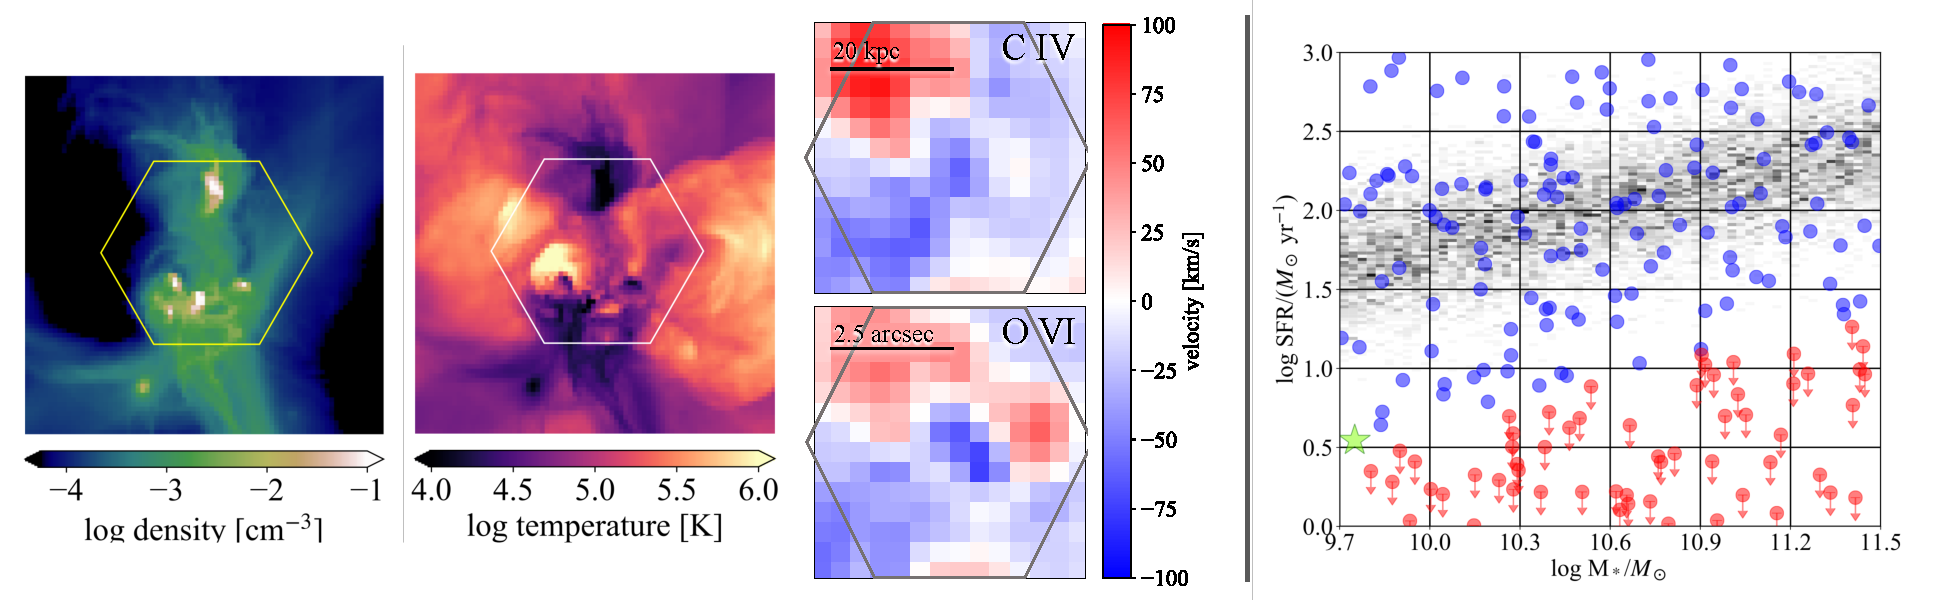
\includegraphics[width=\textwidth]{figs/msipProposalCgmCombo.pdf} 
\caption[CGM simulation examples and proposed sample]{\textit{Left}: Simulations of the density and temperature of the CGM at $z=2-2.5$ based on \citet{Corlies:2018aa}. \textit{Center}: Predicted observations of CGM emission sampled by the FOBOS IFUs, providing kinematic maps that trace gas flows using UV tracers (C IV and O VI).  \textit{Right}: The \textit{FOBOS Galaxy Ecosystem Program} will map these features for hundreds of galaxies sampling a large range physical parameters.  This panel shows a mock sample of program galaxies (star-forming in blue; passive in red) in the stellar mass-star formation rate ($M_*$-SFR) parameter space; the example simulation shown to the left is marked by a green star. The $M_*$-SFR ``main sequence'' from \citet{Whitaker:2012} is shown as the underlying gray 2D histogram.}
\label{fig:cgmsample}
\end{figure}

% In longer term, think through science that we should be proposing now-ish to do with JWST with the idea that we can follow-up with FOBOS.

% Billion galaxy survey?
%Field selection will take advantage of quasar-quasar pairs 
%at \note{range or exact number?} certain redshifts.

% In a joint observing scheme with the ultra-deep exposures of the \textit{FOBOS Cosmology Program}, the CGM study would use FOBOS's unique IFU multiplex capability (configuring one-third of FOBOS's fiber complement into into 15 37-fiber IFUs) to build an unprecedented sample of galaxies spanning respectively $\sim2$ and $>3$ orders of magnitude in $M_\ast$ and SFR, with maps of their CGM \textit{in emission}.  Each IFU will observe an on-sky diameter of 5.6 arcsec, sampling gaseous halos in each galaxy at 5 kpc scales out to a radius of 20--25 kpc (Fig.~\ref{fig:cgmsample}).  These observations require the equivalent of 12.5 dark nights per year.

\section{Kilonovae astrophysics}

The joint detection of electromagnetic radiation and gravitational waves from GW170817 began a new era of multi-messenger astronomy.  This single binary neutron star merger and its associated kilonova have transformed our understanding of multiple branches of astrophysics, from the physical nature of mergers and explosion mechanisms to the origin of the heaviest elements in the universe.  By the late 2020s, gravitational wave detectors like LIGO,\footnote{The Laser Interferometer Gravitational-Wave Observatory} Virgo, and KAGRA\footnote{The Kamioka Gravitational Wave Detector, formerly the Large Scale Cryogenic Gravitational Wave Telescope (LCGT)} will routinely detect $\sim$30 binary neutron star mergers with kilonovae (KNe) annually \citep{abbott2018prospects}, providing the samples needed to understand how the physical properties and nucleosynthetic yields of KNe vary with environment.  Rapid spectroscopic follow-up of these events are critical to these studies, particularly for studying quickly decaying phases such as the Lanthanide-free ``blue" component of the KN light curve that peaks within a day post-merger at $\lambda_\mathrm{peak}\sim0.35$ $\mu$m (Fig.~\ref{fig:kilonova}).

Rubin Observatory target-of-opportunity (ToO) observations will search for KNe within an hour after the gravitational wave alerts are issued \citep[assuming the strategy proposed by][]{margutti2018}. For a typical 50 deg$^2$ localization region, we expect $\sim$100 KN candidates with $m_i\lesssim22.5$, the expected KN brightness at a sensitivity distance of 200 Mpc \citep{cowperthwaite2017, goldstein2019}. Identifying and triggering spectroscopic investigations of the true KNe will require rapid and blue-sensitive follow-up capabilities. Such rapid follow-up of KNe candidates discovered by LSST will enable a systematic population study of KNe and their environments.

%, each with a typical localization region of $\Omega_\mathrm{90\%}<100$ deg$^2$ . 

\begin{figure}
\begin{center}
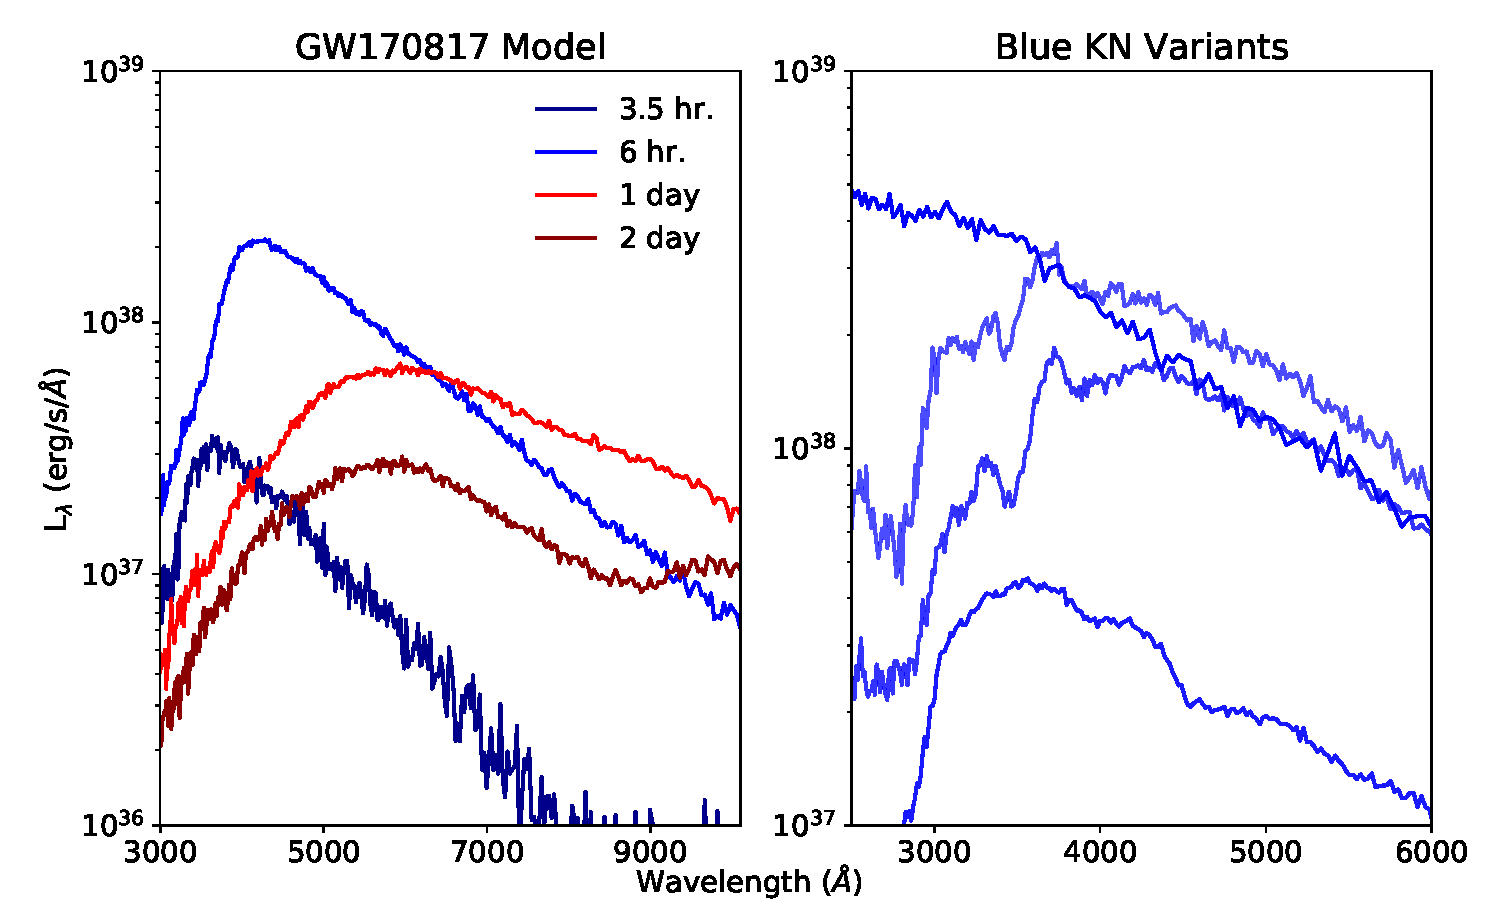
\includegraphics[width=0.8\textwidth]{figs/kn_fobos.pdf}
\end{center}
\caption[Model spectra of kilonovae]{\textit{Left:} Model kilonova spectra based on GW170817 taken 3.5 hours, 6 hours, 1 day and 2 days post-merger. \textit{Right:} Variations of ``blue" kilonovae, generated by varying the energy, mass and Lanthanide fraction of kilonova models. FOBOS's blue sensitivity is essential to discriminate between these early-time models. Models from \citet{kasen2017}.}
\label{fig:kilonova}    
\end{figure}

Building spectroscopy of many KNe can be an expensive endeavor, both because LSST only provides KNe \textit{candidates} that must be spectroscopically vetted and because of their low on-sky density.  It is worth noting, therefore, that a highly multiplexed instrument is beneficial in this case because the KNe spectroscopy can be obtained jointly with other programs; however, this capability is not strictly a requirement of this specific program.

The 12.5 night Kilonovoe Program will vet KNe candidates and ultimately build a sample of high-quality KNe spectra at multiple evolution phases.  

\medskip
\noindent \textbf{FOBOS Kilonovae Program Requirements:}

\begin{programrequirement}
\reqitem Adopting the forecast in \citet{margutti2018}, we expect $\sim4$ bona-fide $z < 1$ KNe to be detectable by LSST and Keck annually. Over the duration of the program, FOBOS will observe $\gtrsim50$ LSST-triggered KNe candidates in the accessible LSST footprint with short ($\sim$10 min), low-resolution ($R\sim1000$) spectroscopy.  This is nearly twice the total spectroscopic follow-up effort currently possible \citep{hosseinzadeh2019}.

\reqitem It should be possible to interrupt any FOBOS program (ToO) and switch to a new field and set of targets within 1 hour of an event trigger.  Efficient target allocation of unused fiber-apertures at the new field location should make use of pre-defined target catalogs, with priority assigned to background targets from the interrupted program.  A software mechanism should allow the ToO observers and the regularly scheduled observers to coordinate the optimal fiber assignment, if desired.


\reqitem Quick-look reductions requiring no more than 2 minutes of runtime should allow for identification of KNe with $m_i < 22.5$ AB.  The goal is 90\% completeness based on 10-minute spectroscopic integrations in average FOBOS conditions. 

\reqitem For confirmed KNe, the program should immediately transition to deeper ($\sim$1 hr) observations to potentially capture ``blue'' KNe (Fig.~\ref{fig:kilonova}).
\end{programrequirement}

%We would observe each candidate with FOBOS's central, fixed IFU to obtain a redshift and potential-host properties.  If our monitoring of real-time quick-look reductions identifies the KN, our strategy would immediately initiate deeper ($\sim1$ hour) observations to potentially capture ``blue" kilonovae   With four KNe annually, this FOBOS program requires $2.5$ nights per year; beyond the KNe observations, many fibers would be allocated to pre-assigned transient sources.

\medskip
\begin{sciencerequirement}
\reqitem Observations should acquire spectroscopy of both the KNe and the host galaxy with an always-deployed integral-field unit (IFU) with an angular diameter greater than 3 arcsec.  This size mitigates modest localization errors.  The resulting datacubes from this IFU should provide spatial sampling that allows independent spectra to be extracted for at least 5 separate regions of a typical $L_*$ host galaxy at $z \approx 0.7$.

\reqitem Candidate vetting spectra must achieve S/N$\sim$3 at a magnitude limit of $g_\mathrm{AB}=24$ to identify KNe at limiting distance of $D_\mathrm{L}\sim300$ Mpc.  \edit{translate into actual KNe brightness of 22.5?}

\reqitem Redshift uncertainties of the host galaxy must be $\sigma_z/z \lesssim0.1$. \edit{this seems absurdly large -- just use a photo-z.  Restate or drop?}
\end{sciencerequirement}

\section{Time-Domain Characterization of Extragalactic LSST Transients and Host Galaxies}

%Each DDF is roughly 9 sq deg

Beyond KNe, Rubin Observatory will discover well over 1 million extragalactic transients annually, including thousands of currently rare sources such as tidal-disruption events \citep{bricman2020}, superluminous supernovae \citep{villar2018} and changing look quasars.  The on-sky densities are such that we expect $\sim$5 LSST transient hosts per 20\arcmin\ field-of-view.  Within the LSST Deep Drilling Fields observed by FOBOS for the {\it FOBOS Cosmology} and {\it Galaxy-Ecosystem Programs}, we expect $\sim$150 total transients to be visible each year with $m_i<24$. For a highly multiplexed instrument with dynamic target allocation, a high-impact, low-cost strategy would be to follow-up \textit{every} LSST transient and transient host within any given Keck pointing. Currently, roughly 1,000 supernovae have spectroscopic observations each year, although essentially all are observed at $m_i<21$. By combining both single-aperture and IFU observations of transients, we would dramatically increase the database of transient spectroscopy for low-luminosity events.  In particular, IFU observations of this regularity would dramatically increase the resolved spectroscopy of extragalactic hosts \citep[see a recent review by][]{anderson2015} at little additional cost. A series of requirements follow for observations of these targets:


\medskip
\noindent \textbf{FOBOS Transients Program Requirements:}


\begin{programrequirement}
\reqitem This program would reserve 5--10 single-aperture fibers in specified FOBOS pointings within the LSST footprint that are to be observed by other FOBOS programs.  

\reqitem It should be possible to assign or adjust the on-sky targets for these reserved fibers in as little as 15 minutes before acquiring a new field configuration.

\end{programrequirement}

\medskip
\begin{sciencerequirement}
\reqitem A central IFU with a minimum field-of-view of 3\arcsec\ should be continuously deployed in all FOBOS instrument configurations.

\reqitem UV sensitivity to the atmospheric limit (310 nm) as rest-frame $\lambda \lesssim 0.3$~nm is required for studying shock-driven (e.g., Type IIn supernovae) and relativistic events \citep[e.g., the atypically bright Type Ib supernova AT 2018cow;][]{margutti2019}.

\reqitem The widest possible simultaneous wavelength range to study a broad range of host galaxy redshifts and spectral features associated with transient phenomena.  
\end{sciencerequirement}

% By deploying the remaining single fibers and IFUs on separate, pre-assigned transient sources in each pointing, we will take maximum advantage of synergies with time-series data from the world-wide follow-up observations of these gravitational-wave fields. 

% When deployed as the Keck II instrument, FOBOS's always-ready IFU makes it ideal for instant target acquisition and host galaxy characterization, all while simultaneously observing serendipitous targets of interest in the same field-of-view. 


\section{Chemodynamical Evolution of the M31 and M33 Disks}
\label{sec:m31disk}

\begin{figure}
\begin{center}
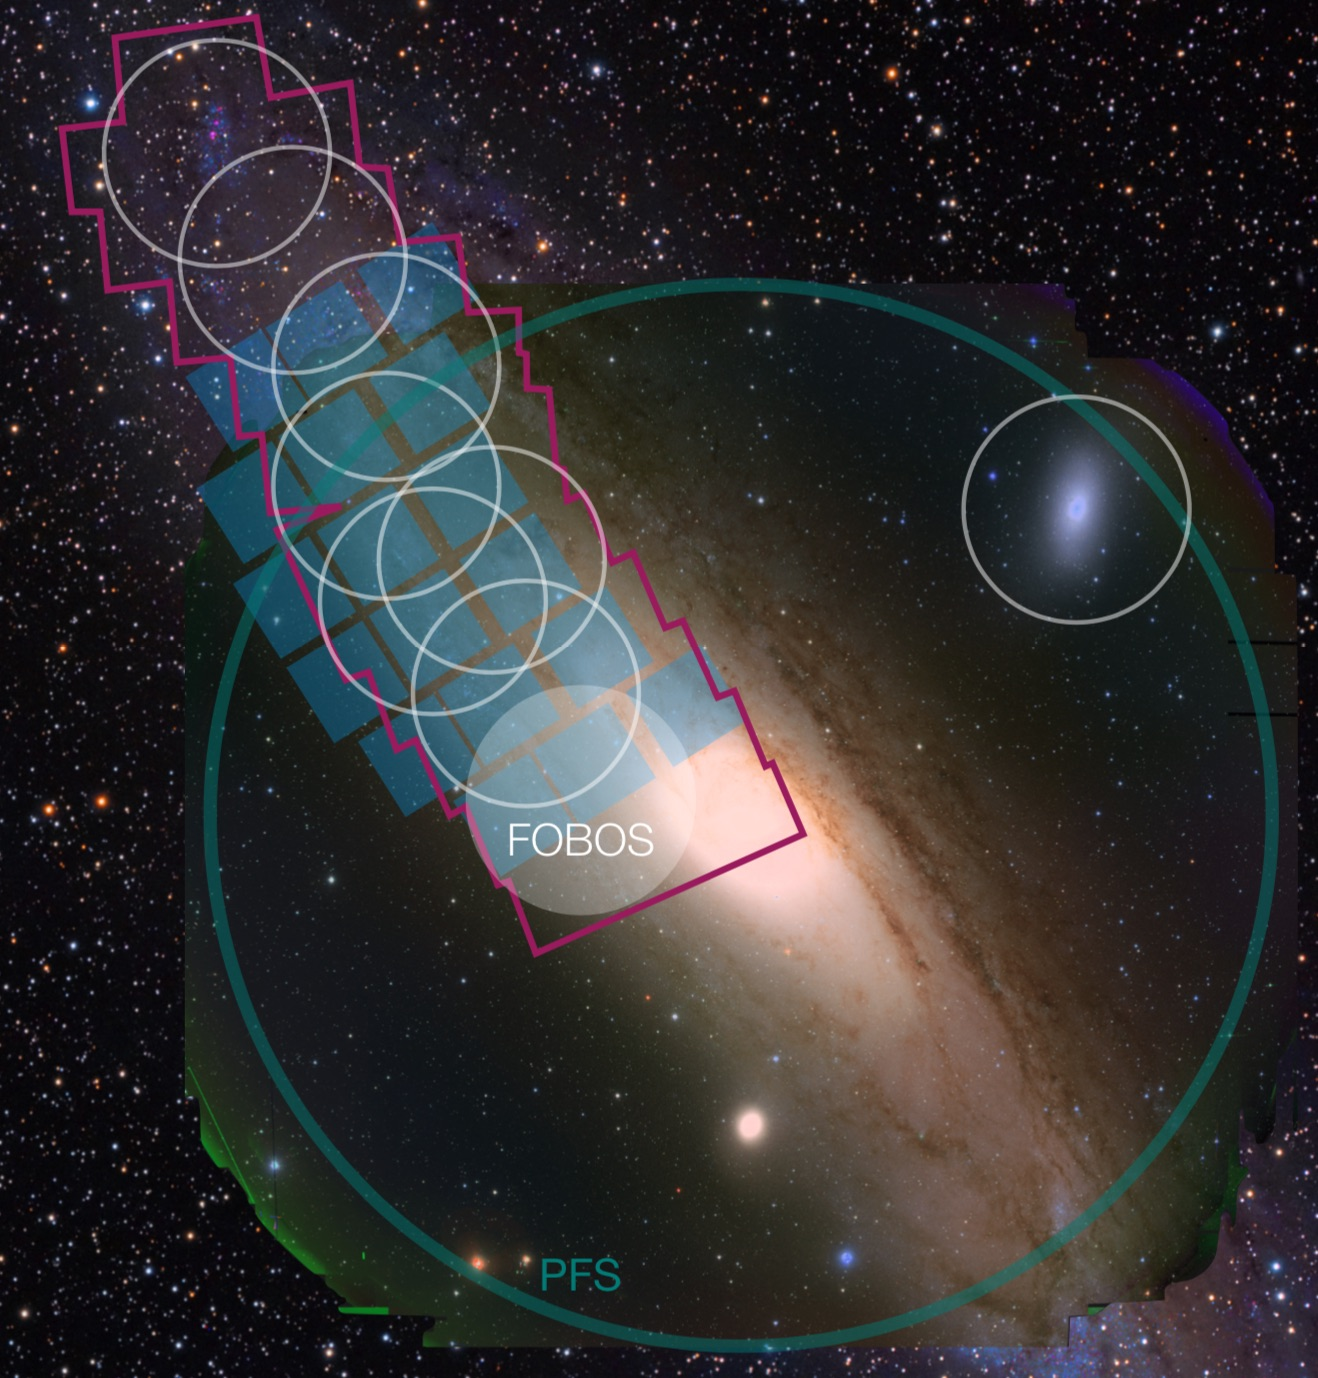
\includegraphics[width=0.58\textwidth]{figs/M31_footprint_v3.jpg}
\end{center}
\caption[M31 pointing distribution]{A Subaru HSC image (lower right) superposed on a larger background image of M31 (credit: Adam Evans).  Keck II Nasmyth pointings (white circles) can be arranged to span the PHAT area (magenta) and NGC 205.  The Subaru-PFS FOV (green circle; similar to MSE) and single-pointing WFIRST imaging footprint (blue squares) are also shown.}
\label{fig:M31}    
\end{figure}

Galaxy groups like the Local Group, with two L$^*$ galaxies, dominate the nearby universe \citep{kourkchi17}.  We expect galaxies in such groups to share common assembly histories, and yet, the Milky Way and Andromeda galaxies (M31) appear to have evolved in significantly divergent ways.  Differences from their star-cluster populations to their dwarf-galaxy properties remain poorly understood, limiting progress towards building a complete picture for how the Local Group formed and evolved.

For the Milky Way, stellar properties (e.g., age, metallicity, $\alpha$ abundance) and kinematics from large-scale spectroscopic surveys (e.g., APOGEE, GALAH, LAMOST) are now being combined with exquisite astrometric data from \textit{Gaia} to provide a revolutionary view of its evolution.  For example, these data reveal a clear bimodality in $\alpha$ abundance, indicating that stars at relatively greater distances from the disk plane (i.e., ``thick-disk'' stars) were formed in environments with much shorter star-formation timescales, likely due to a merger event that truncated star formation for a time. This is further confirmed by spectroscopic ages of the stars derived via data-driven methods which tie spectral CN features to their asteroseismic ages \citep[e.g.][]{Martig16}.  Isolating chemically similar groups of stars in this way to reveal their common structural and dynamical properties is now fundamental to our understanding of the Milky Way.  This ``chemical tagging'' offers greater insights than studies of stars selected by their structural or dynamical associations alone \citep[e.g.,][]{Ting15}.  The next stage in understanding the Local Group should apply similar methods to the study of M31 and its satellite galaxies.

If we can obtain large samples of stellar spectra ($\gtrsim 10^5$) in the disk of M31, we can map the velocity dispersion of populations of different ages and metallicities by position in the galaxy for detailed quantitative comparisons to simulations of M31's interaction and merger history. Although chemical tagging with M31 benefits from our outside view (compared to our inside view of the Milky Way), it also faces the challenge of obtaining precise stellar parameter measurements for very large samples.  First steps were made by SPLASH,\footnote{Spectroscopic and Photometric Landscape of Andromeda’s Stellar Halo \citep[e.g.][]{splash}} which obtained $\sim$1hr Keck-DEIMOS exposures for $\sim$10,000 RGB stars in the disk, stellar streams, and halo of M31.  \citet{dorman15} used SPLASH to study the stellar age and velocity dispersion of disk stars and found that M31 features a much thicker, high-dispersion component compared to the Milky Way.  More recently, \citet{escala20} explored metallicity and $\alpha$ abundance trends in 70 RGB stars ($\sim$6hr Keck-DEIMOS integrations) in the outer disk, inner halo, and Giant Stellar Stream of M31.  These trends also suggest a significant, merger-induced star-formation event in M31.  However, without more precise stellar parameters and larger samples --- beyond the limits of what one can expect to achieve with DEIMOS --- we can only determine general trends in the overall populations.  With the order of magnitude increase in sample size and factor of {\bf XXX} increase in parameter and velocity precision achievable due to FOBOS's blue sensitivity, we can make clear distinctions between populations with different metallicity and spatial distributions that contrast the evolutionary histories of the Milky Way and M31 disks and satellite population.

\begin{figure}
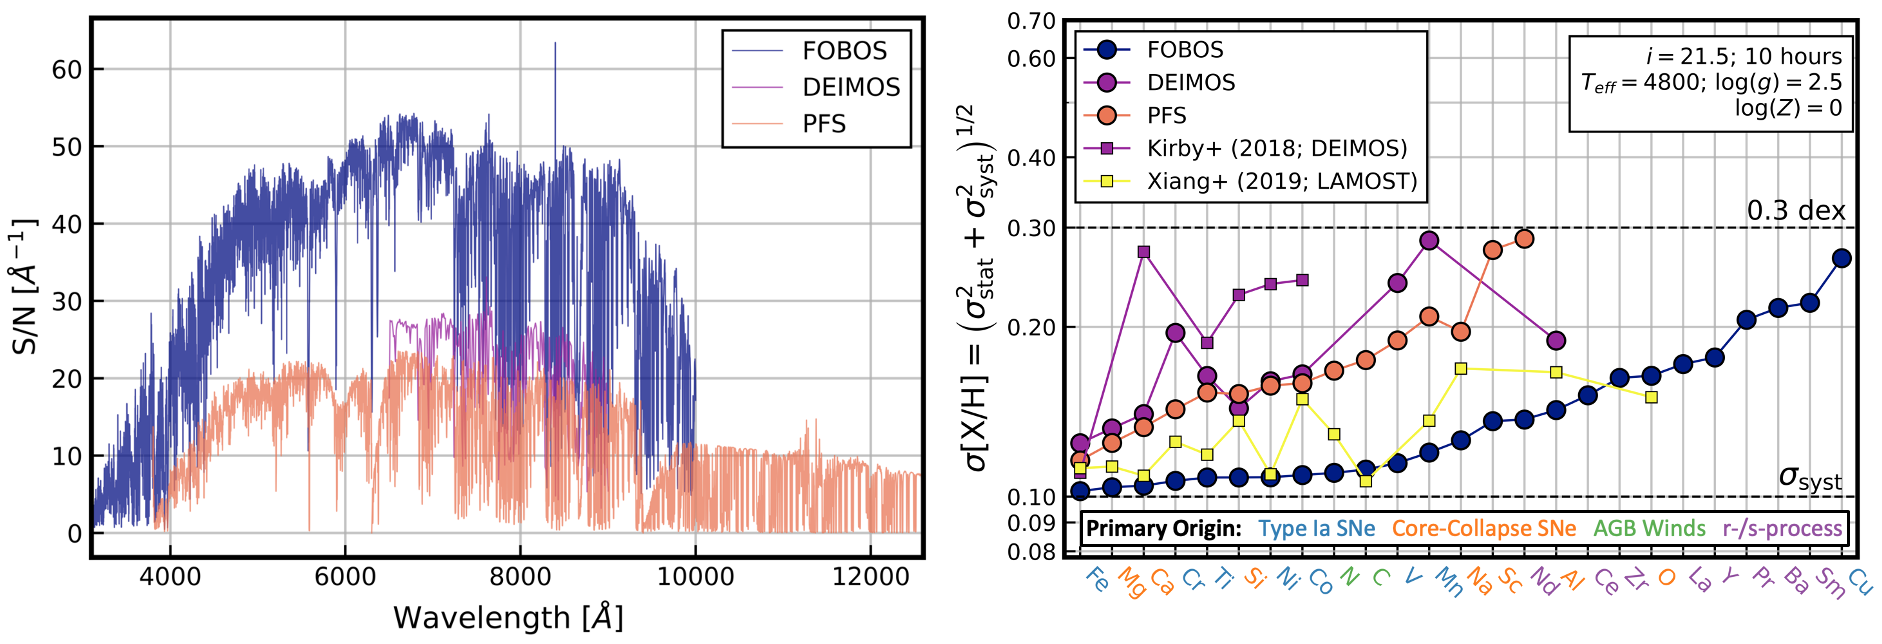
\includegraphics[width=1.0\textwidth]{figs/abundances_snr_v6.png}
\caption[Simulated M31 RGB spectra and abundance forecasts]{Simulated observations demonstrating FOBOS's ability to perform ``chemical tagging'' in M31 and M33. \textit{Left:} Expected S/N for an $i=21.5$ RGB star in M31 observed for 10hr using FOBOS, PFS, and DEIMOS. \textit{Right:}  Forecasted abundance precision for these observations (filled circles), including both statistical uncertainty ($\sigma_{\rm stat}$; predicted by the Cram\'er-Rao Lower Bound) and a 0.1-dex systematic uncertainty \citep[$\sigma_{\rm syst}$; cf.,][]{kirby18, xiang2019}. Elements are ordered along the ordinate by decreasing precision (limited to $\lesssim$0.3 dex) and color-coded by their primary nucleosynthetic origin. Although these forecasts are optimistic, the indicated \textit{relative} precision between instruments is robust. For reference, we show abundance uncertainties reported by \citet[][purple squares]{kirby18} from DEIMOS spectra of $-1.0<\text{[Fe/H]}<-0.6$ RGB stars in MW satellites with comparable S/N to our simulations; their measurement precision is worse than our DEIMOS predictions primarily because of their lower metallicity targets.  We also show abundance uncertainties reported by \citet[][yellow squares]{xiang2019} from LAMOST spectra of MW RGB stars, scaled to the S/N and resolution of the proposed FOBOS  observations.}
\label{fig:abundances_snr}
\end{figure}

We have therefore developed the following program to provide the first clear, spatially-resolved measurements of chemodynamical trends in the M31 and M33 disks, allowing us to address two key questions for the first time: Does M31, like the Milky Way, exhibit its own [$\alpha$/Fe] bimodality?  If so, were the ancient merger histories of the two galaxies linked or largely independent? This program will also increase the number of stars in M31 satellites with precise chemical abundances by two orders of magnitude \edit{check}, enabling\edit{...}  The program requirements are as follows:

\begin{programrequirement}
\reqitem To create 5 bins in age, abundance, and velocity pattern, the stellar sample should be $\sim 10^5$ stars in the M31 disk and $\sim 10^4$ stars in the M33 disk. \label{prog:lgdisks:sample} \edit{does the pre-amble adequately motivate observing the satellites?}.  

\reqitem Six M31 disk fields at radii between 5--20 kpc with two additional fields beyond 20 kpc should be drawn from the PHAT\footnote{Panchromatic Hubble Andromeda Treasury \citep{phat} is a multi-cycle HST program that maps $\sim1/3$ M31's star-forming disk in 6 filters.} HST footprint.  

\reqitem The total number of M31 FOBOS-visits is 64 with 10-hour integrations required per visit.  Given rejections due to crowding \citep{dorman12} of RGBs at ($i_{\rm Vega} < 22.5$), a science-fiber multiplex of at least 1600 per pointing is required to build the M31 disk sample of $\sim 10^5$ stars.

% K. Bundy (2021-04-07): Commenting these out because they don't impact FOBOS instrument design.
% \reqitem All stars should be observed over a region with high resolution photometry for targeting fidelity.
% \reqitem Target selection should account for precursor/coincident surveys planned with Subaru PFS and the Maunakea Spectroscopic Explorer (MSE).


\reqitem To build the necessary M33 disk sample (\ref{prog:lgdisks:sample}), we require 3 fields each visited twice.
\reqitem To build the necessary M31 satellite sample (\ref{prog:m31halo:sample}), we require 3 fields in the region including NGC 147, NGC 185, and And II, each visited once, and 1 pointing in NGC 205, visited twice.  


\reqitem To maximize observing efficiency, each disk field should achieve $\sim$95\% efficiency of allocated spectrograph apertures \edit{check; basically we want to max this out}.


\reqitem To enable robust and informative modeling of the M31 satellite system's chemodynamical evolution, the stellar sample should be $\sim10^{4}$ RGB stars across multiple M31 satellite galaxies.  \label{prog:m31halo:sample}

\end{programrequirement}

\medskip
\begin{sciencerequirement}
\reqitem The velocity precision of each star observed should be $\lesssim 5$ \kms.
\reqitem In M31 and M33, The abundance precision must be $\sim 0.1$ dex for both [Fe/H] and [$\alpha$/Fe]; additional abundances for individual elements produced via Type Ia SNe (e.g., Cr, Ti, Ni), core-collapse SNe (e.g., Mg, Ca, Si), and various proposed neutron-capture channels (e.g., Nd, Y, Ba) should be measured to $\sim$0.2 dex \citep[Fig.~\ref{fig:abundances_snr}; cf.][]{Sandford20}. \label{prog:lgdisks:precision}
\reqitem In M31 satellites, the abundance precision must be $\lesssim 0.2$ dex for both [Fe/H] and [$\alpha$/Fe].
\reqitem Stellar ages for M31 and M33 disk stars must be attainable to 0.1 dex via, e.g., use of the blue CN absorption features \citep[e.g.][]{Martig16,Ting19}.  %This typically requires S/N $\approx$ 30 per pixel at $R=1800$.
\label{prog:age:precision}
\reqitem To achieve the required measurement precision (\ref{prog:lgdisks:precision}, \ref{prog:age:precision}), we must reach an $i$-band ${\rm S/N} \approx 40$ \AA$^{-1}$ and $\approx 20$ \AA$^{-1}$ at the  ``sweet-spot'' of the RGB ($i_{Vega} = 21.5$) and a magnitude fainter, respectively, in $\sim$10 hours.  This assumes a resolution of $R\sim3000$ and a wavelength coverage from 0.3 -- 1$\mu$m.
\end{sciencerequirement}

\section{Young star clusters in the disk of M31}

\edit{Need a few motivating sentences here about the scientific gain of these observations.  Emphasize need of IFUs for local background subtraction.  Blue response needed to capitalize on young, blue stars (included among requirements below).  Move discussion of joint observations to separate section.  }
The M31 disk contains thousands of young star clusters.  These clusters probe the process of star formation throughout the many environments present in the disk, including the clusters' dynamics and chemistry, as well as the conditions under which stars are formed and dispersed throughout the disk.  Although insights into the recent evolution of the M31's disk have already been possible through their photometric properties \citep[e.g.,][]{johnson16}, FOBOS will provide abundance, velocity, and mass information that is currently unavailable, allowing both confirmation of the inferences from photometry as well as large samples of spectroscopic masses and abundances to track the recent formation of stars and metals in clusters across the disk. Jointly with single-fiber observations of RGB stars, we would acquire IFU observations ($\sim$5.6\arcsec{} diameter), comparable to the sizes of $\sim$500 \edit{check} young star clusters in the M31 disk classified by the Panchromatic Hubble Andromeda Treasury \citep[PHAT;][]{johnson15}.  This legacy campaign would dwarf even Milky Way samples of young star clusters \citep{johnson15}.  In particular, observations of young stellar clusters require blue sensitivity and IFU capabilities to produce integrated-light spectra of these objects used to probe the recent evolution of the star-forming disk. Many of these star clusters are loose enough that the massive stars they contain can be resolved individually or in small very compact groups within the cluster.  IFU spectroscopy will provide optimal spatial resolution to separate these components to probe both the velocity dispersions and metallicities of the clusters.  Moreover, as the ages of these clusters are well-constrained from PHAT resolved stellar photometry, we can tie measurements of the cluster velocity dispersion to its age to constrain their dynamical evolution.  Finally, we can also integrate the IFU spectra to test our ability to measure ages and metallicities of young clusters with integrated light FOBOS spectra in more distant galaxies.

\edit{cluster size benefits significantly from IFUs because of close packing!}

\begin{programrequirement}

\reqitem Acquire a sample of 500 young stellar clusters to probe different regions of the M31 disk and different cluster properties.
\reqitem Sensitivity below 6000 Angstroms required to detect bright continuum and absorption features from the young main-sequence stars.
\reqitem Velocity precision high enough to make dispersion measurements for typical young clusters.\YST{maybe be more specific?} \edit{How many stars do we expect per cluster, or is the velocity dispersion going to be from an integrated light spectrum?  Typical cluster dispersion is $\sim 5-10$ km/s? $R\sim3500$ is an instrumental resolution of $\sim$36 km/s, so measuring dispersions for integrated light spectra to $\sim$20 km/s will be tough. Recast as a goal.} 
\reqitem IFU observations are required to differentiate the integrated cluster light from the background of M31's disk.
\reqitem IFU observations are required to measure velocity dispersions.
\end{programrequirement}

%the blue sensitivity of FOBOS, along with its ability to obtain many small IFU regions within each pointing, will provide detailed spectroscopic maps of $\sim$500 young star clusters, , portegies10.  These clusters probe

% , including its dynamics and chemistry, as well as the conditions under which stars are formed and dispersed throughout the disk.  Although insights into the recent evolution of the M31's disk have already been possible through their photometric properties \citep[e.g.,][]{johnson16}, FOBOS will provide abundance, velocity, and mass information that is currently unavailable, allowing both confirmation of the inferences from photometry as well as large samples of spectroscopic masses and abundances to track the recent formation of stars and metals in clusters across the disk. 

% Wide-field ($\sim$20 kpc at M31 distances) mapping of the M31 halo, using instruments like PFS and MSE,\footnote{The Maunakea Spectroscopic Explorer (MSE) is a concept being developed for a future telescope and instrument at the current Canada-France-Hawaii Telescope site.} will soon probe the chemodynamical history of its stellar substructures; however, FOBOS will provide unique capabilities particularly suited to the high-source-density M31 disk (see Fig.~\ref{fig:M31}).

% However, FOBOS's blue sensitivity, order-of-magnitude greater sampling density, and IFU modes offer  unique capabilities for obtaining a high-source-density census of M31's disk (see Fig.~\ref{fig:M31}), M33, and the cores of Andromeda's major satellites.  Such data enable the chemodynamical studies needed to address key questions about the structure and assembly of these objects. 

%These relations will determine whether M31's thicker disk is the result of dynamical ``heating'' of stars initially formed in a cold, thin disk versus the ``settling'' of a more turbulent primordial disk into the dynamically cold structures seen today.

%Our large sample size, more than an order of magnitude larger than currently available, will allow for the finer subdivision of the stellar populations and the more-detailed quantification of the chemodynamical structures in M31 and M33, needed for a robust comparison to similar structures in our Milky Way.  

%Currently, {\it only} the Milky Way disk has been measured with this kind of precision, and it required very large surveys with substantial resources to complte, such as LAMOST  \citep{xiang2017, Xiang2019} and APOGEE \citep{hayden2015}.  With FOBOS, we can add {\it two} more disks to this detailed sample as just one example program of the science enabled.

%\note{Yuan-Sen: Maybe a sentence or two summarizing the importance of age-velocity-dispersion relation: e.g., nature vs. nurture; upside down ISM cooling vs. secular evolution}

%\note{Yuan-Sen: PHAT CMD + FOBOS spectra should give pretty good spectroscopic-photometric constraints on stars}

%\note{note gains in RGB numbers by probing deeper down the sequence?} 

% Proof in the pudding:
%\note{ref; https://arxiv.org/abs/1908.09727 ?}.

%----------------------------------------------------------
\section{Milky Way dwarf galaxy dynamics and the search for Dark Matter}

\edit{copied from msri pre-proposal}
Nearby dwarf galaxies ($<$ 1 Mpc) can be resolved into individual stars, providing great potential as laboratories for testing theories of galaxy formation and fundamental physics.  Deep-and-wide imaging from Rubin and Roman will open a new chapter in this field by detecting new dwarf galaxies and dramatically improving our census of member stars in known systems.  Once again, the addition of uniquely deep, high-multiplex FOBOS spectroscopy will allow the full potential of LSST/Roman dwarf galaxy observations to be realized.  This combination will have a major impact on the astrophysical search for dark matter in the next decade \citep{drlica-wagner19}.  Ideally suited as described by \citet{simon19} because of its FOV, sensitivity, and unrivaled efficiency at target separations down to 10\arcsec, FOBOS builds on the legacy of Keck-DEIMOS that has dominated dwarf galaxy spectroscopy over two decades.  Reaching 0.5 mag fainter than DEIMOS with twice the bandpass and 20 times the multiplex, FOBOS will play two important roles in the search for dark matter using dwarf galaxies.  First, FOBOS will spectroscopically confirm an anticipated $\sim$200 new low-luminosity dwarf candidates to constrain the ``minimum halo mass'' cutoff in the subhalo mass function as predicted by warm dark matter (WDM) models and other variants (e.g., `fluid', `fuzzy', `wave-like').  \citet{jethwa18}, for example, establish a WDM limit of $M_{\rm WDM} > 2.9$ keV based on the currently known Milky Way dwarf population while \citet{nadler19} extend a similar analysis to derive a 95\% upper bound of $6 \times 10^{-30}$ cm$^2$ for the DM-baryon cross section at 10 keV.  FOBOS confirmation of a highly complete LSST/Roman subhalo sample will deliver order-of-magnitude improvements in mass and cross-section limits by eliminating nuisance parameters on the galaxy-halo connection and subhalo disruption fraction.

Second, FOBOS will place tight limits on the cross section of self-interacting dark matter (SIDM) models by increasing the number of highly sampled dwarf galaxy density profiles by 1--2 orders of magnitude.  Currently, the best limit of $\sigma_{\rm SIDM}/m < 0.32$ cm$^2/$g (assuming velocity-independent SIDM) comes from a single dwarf galaxy, Draco, with 500 kinematic tracers \citep{read18}.  FOBOS will select targets from LSST/Roman imaging to go deeper down the RGB luminosity function and obtain $>$1,000 tracer stars at 1 km s$^{-1}$ precision for each of 50 Local Group dwarfs \citep[see][]{drlica-wagner19}, pushing the $\sigma_{\rm SIDM}/m$ bound to 0.05 cm$^2/$g and enabling exploration of more complex SIDM dynamics.  The sample will include both Milky Way satellites and M31 dSphs (with tracers selected from Roman), whose compact nature requires FOBOS's high sampling density.   

The FOBOS-derived dwarf galaxy density profiles are also critical to indirect detection searches for weakly interacting massive particle (WIMP) candidates such as Majorana fermions that produce pair annihilation gamma rays.  This is because the gamma-ray flux is proportional to the integral of the square of the density profile (the $J$-factor), in addition to its dependencies on particle cross section and mass.  Using a Fisher matrix approach, we estimate that our FOBOS program will improve existing $J$-factor measurements for classical dwarfs by a factor of 5.  Adding new FOBOS $J$-factors for additional dwarfs will bring further gains.  Even with existing Fermi LAT detection limits, our program would push current WIMP cross section upper bounds an order of magnitude lower to 10$^{-25}$ cm$^3$ s$^{-1}$ at 5 GeV.

\medskip
\noindent \emph{Impact Summary:} \textbf{FOBOS will yield order-of-magnitude improvements in cross-section and particle-mass limits across multiple, disparate regions of the proposed dark matter parameter space}.  The fact that state-of-the-art direct detection experiments offer such gains in just one part of parameter space, at a cost of \$60-100M each, demonstrates how powerful and cost-effective is FOBOS spectroscopy (combined with LSST/Roman imaging) in the search for dark matter.

\section{Machine Learning}

\edit{Not really a key program, but I put this section here mostly as a reminder to think about how we can incorporate those ideas into this document.}

Think of this the other way around, as well.  Because Astronomy is data wealthy, that enables development of new machine learning tools/methods.

Homogeneity and repeatibility.  Work it backwards to what development the machine learning applications need.

Ease of access (things not only available as fits files), populate a database that is more accessible programmatically.  Cloud computing capabilities.  Avoid having multiple copies distributed across users.

Machine learning application for operational part.

\newpage


%%%%%%%%%%%%%%%%%%%%%%%%%%%%%%%%%%%%%%%%%%%%%%%%%%%%%%%%%%%%%%%%%%%%%%%%
% Technical Requirements
%%%%%%%%%%%%%%%%%%%%%%%%%%%%%%%%%%%%%%%%%%%%%%%%%%%%%%%%%%%%%%%%%%%%%%%%

\chapter{Instrument Requirements}
\label{chap:instr}

\edit{need a scheme for translating P, S and R, D to things like TOP.REQ.A01 for the requirements tables}

Summaries of Science and Program requirements and how they flow down to technical requirements.

To be populated from Wiki Tables: \url{https://uco.atlassian.net/wiki/spaces/FOB/pages/15990810/Requirements}

\section{Spatial Sampling}
\label{sec:sampling}

\medskip
\noindent The main requirement on spatial resolution is that the delivered effective PSF shall not be degraded by more than 60\% from typical site conditions at all wavelengths:


\begin{requirement}

\reqitem The shape of the IFUs will be hexagonal as a best approximation of a circular aperture with natural fiber-packing and regular perimeter for mechanical mounting.

\reqitem The size and number of IFUs shall be determined by ...

\reqitem The FWHM of unresolved (stellar) objects in the reconstructed data cubes shall be 2.5\arcsec\ or less at $\lambda = 5400$ \AA\ in median observing conditions (1.5\arcsec\ seeing).

\reqitem The observational PSF of the reconstructed data cube must be circular at all locations to a tolerance of $b/a > 0.85$, with $b/a$ the observed axis ratio.

\reqitem The angular resolution of any spatial element within the reconstructed data cube shall not vary by more than 10\% from the average at any given wavelength, i.e., the effects of differential atmospheric refraction on the sampling must be wavelength-independent at this level.

\end{requirement}

\section{Spectrophotometry}
\label{sec:spectrophotometry}

The science requirements for spectrophotometry are driven by two considerations: (1) the need to derive accurate physical parameters from the widely-spaced nebular emission lines, e.g., SFR, dust attenuation, metallicity; (2) the need to derive accurate physical parameters from the stellar continuum through stellar population synthesis. This translates into the following requirements:

\begin{requirement}

\reqitem Relative spectrophotometry to 2.5\% between \Halpha\ and \Hbeta.
    
\reqitem Relative spectrophotometry to 7\% between [OII]$\lambda3727{\rm \AA}$ and [NII]$\lambda6584{\rm \AA}$. 
    
\end{requirement}

\subsection{Justification}

Following \citet{kennicutt1998} and \citet{calzetti01}, to achieve 5\% errors on the SFR from \Halpha\ we require a maximum 2.5\% error on the Balmer decrement. This ensures we are never dominated by spectrophotometric errors.

An important scientific goal is to measure nebular metallicity gradients. These are typically quite shallow, of order $\sim0.04$~dex/kpc \citep{vanzee1996}. It is thus desirable to have our spectrophotometry errors contribute no more than 0.01 dex to the error budget. The [N~II]6584~/~[O~II]3727 line ratio is one of the best lines for metallicity measurement in moderately metal-rich nebulae ($12 + \log(\mathrm{O/H}) > 8.5)$ due to its independence on the ionization parameter \citep{kewley02}. We can achieve a $\sim0.01$~dex error in metallicity with a less than 7\% error in the relative spectrophotometry between [OII] and [NII].

%%%%%%%%%%%%%%%%%%%%%%%%%%%%%%%%%%%%%%%%%%%%%%%%%%%%%%%%%%%%%%%%%%%%%%%%
% Guiding
%%%%%%%%%%%%%%%%%%%%%%%%%%%%%%%%%%%%%%%%%%%%%%%%%%%%%%%%%%%%%%%%%%%%%%%%
\section{Guiding and PSF Metrology}
\label{sec:guiding}

The high-level requirement is that guide errors should not dominate the positional error and image quality degradation of the target galaxies within the bundles. This leads to two specific requirements:

\begin{requirement}

\reqitem Guiding accuracy should be no worse than 0.2\arcsec.
    
\reqitem Knowledge of the PSF across the plate should be no worse than 0.2\arcsec.
    
\end{requirement}

\subsection{Justification}

The stack-up of mechanical tolerances in the ferrules, holes, and the plugging process, the plate shape errors, and the alignment of the bundles w.r.t.\ the chief ray leads to a guide accuracy requirement of 0.2\arcsec.

PSF metrology across the field is crucial for optimal data cube extraction. With our nominal 3-point dither pattern, the reconstructed PSF uniformity across a bundle is $\sim 0.15$\arcsec\ RMS. Mechanical tolerances in ferrule alignment and  the shape of the focal plane cause variations of the PSF of the order of 0.2\arcsec. Hence, for data quality to not be limited by PSF kernel mismatch (used in the extraction),  we require knowledge of the PSF across the field to a similar level.

\section{Program overlap and synergies}

\edit{This section highlights the overlap of the different programs and shows how they can be integrated.  Think Table 2 from the MSIP and the discussion around it.}

\section{Requirements tables}
\subsection{FOBOS.TOP: Top-Level Instrument Requirements}

\begin{description}

\item [TOP.REQ.A01] Field of view (FoV) shall be 17\arcmin{} diameter with a goal of the full unvignetted 20\arcmin{} diameter.  A wider FoV increases the efficiency of targeting sources with lower on-sky densities, thus expanding FOBOS's science breadth.

\item [TOP.REQ.A02] Number of single fibers shall be at least 1800.  Over a 20\arcmin{} field, this number yields an average target density of 6 arcmin$^{-2}$ which matches the desired target density of our Design-Reference Programs.  Note that the on-sky density of sources brighter than i$_{AB}$ $\sim$25 is $\sim$40 arcmin$^{-2}$.

\item [TOP.REQ.A03] The Single-fiber on-sky aperture shall be between 0.7--1.2\arcsec{}.

\item [TOP.REQ.A10] In all instrument modes, FOBOS shall deploy 12 7-fiber bundles (4 per spectrograph) to achieve simultaneous spectrophotometry \citep[see][]{yan16}.  

\item [TOP.REQ.A04] In all instrument modes, FOBOS shall deploy a fixed, central fiber-bundle IFU with an on-sky aperture of 3\arcsec{} diameter.

\item [TOP.REQ.A05] For science and calibration IFUs, individual spatial sampling within the IFU shall correspond to size of 0.33\arcsec{} in order to adequately sample seeing of FWHM$ = 0.6$\arcsec.

\item [TOP.REQ.A06] The 1st-light IFU mode shall deploy 25 fiber-bundle IFUs each composed of 61 fibers.  The format is fixed because galaxy samples with $z > 0.4$ have a relatively confined apparent size distribution with a median of  $\sim$1.5\arcsec{} diameter.

\item [TOP.REQ.A07] The FOBOS 1st-light spectrographs shall span a wavelength range of 0.31-1.0 $\mu$m.  This ensures adequate coverage of spectral features for key program targets and makes sure that FOBOS has no ``redshift desert.''

\item [TOP.REQ.A08] The mid-channel spectral resolution in each spectrograph channel shall reach $R = 3500$

\item [TOP.REQ.A09] Excluding the telescope and atmosphere, the instrument throughput shall be greater than 30\% over 95\% of the full wavelength range.

\end{description}

\subsection{FOBOS.ADC: Atmospheric Dispersion Corrector Requirements}

\subsection{FOBOS.AGS: Acquisition and Guiding System Requirements}

\subsection{FOBOS.FPM: Focal Plane Motion System Requirements}

\subsection{FOBOS.FFP: Fiber Positioning System Requirements}

\subsection{FOBOS.FBR: Fiber System Optics Requirements}

\subsection{FOBOS.SPEC: Spectrograph Requirements}
\subsection{FOBOS.SUPT: Support Systems Requirements}
\subsection{FOBOS.CAL: Calibration System Requirements}
\subsection{FOBOS.DMS: Spectrograph Requirements}
\subsection{FOBOS.OPS: Operations Requirements}

%%%%%%%%%%%%%%%%%%%%%%%%%%%%%%%%%%%%%%%%%%%%%%%%%%%%%%%%%%%%%%%%%%%%%%%%
% Data Requirements and documentation : MOVED TO DATA MANAGEMENT SYSTEMS DOCUMENT
%%%%%%%%%%%%%%%%%%%%%%%%%%%%%%%%%%%%%%%%%%%%%%%%%%%%%%%%%%%%%%%%%%%%%%%%

\newpage

\chapter*{Acknowledgments}
\addcontentsline{toc}{chapter}{Acknowledgments}

FOBOS as a concept was originally developed by Khee-Ghan Lee (IPMU) and David Schlegel (LBNL).  We are deeply indebted to all the scientists that have contributed toward the development of science programs for FOBOS, including (but not limited to): \edit{...}

\newpage

%% Chapter
\chapter*{Revision History}
\addcontentsline{toc}{chapter}{Revision History}

\begin{table}[hp]{%
\begin{tabular}{l | l | l |  p{22pc}} \toprule
\textbf{Version} & \textbf{Date} & \textbf{Editor} & \textbf{Comments} \\ \midrule
% Insert your own version number with the date, your name, and a short
% description of this version of the document.
0A & 2020-09-17 & Kyle Westfall & First draft \\ \bottomrule
\end{tabular}}
\end{table}

%%%%%%%%%%%%%%%%%%%%%%%%%%%%%%%%%%%%%%%%%%%%%%%%%%%%%%%%%%%%%%%%%%%%%%%%
%%%%%%%%%%%%%%%%%%%%%%%%%%%%%%%%%%%%%%%%%%%%%%%%%%%%%%%%%%%%%%%%%%%%%%%%

\bibliography{ref}

\end{document}

% DOCUMENT ENDS HERE!
%%%%%%%%%%%%%%%%%%%%%%%%%%%%%%%%%%%%%%%%%%%%%%%%%%%%%%%%%%%%%%%%%%%%%%%%
%%%%%%%%%%%%%%%%%%%%%%%%%%%%%%%%%%%%%%%%%%%%%%%%%%%%%%%%%%%%%%%%%%%%%%%%
%%%%%%%%%%%%%%%%%%%%%%%%%%%%%%%%%%%%%%%%%%%%%%%%%%%%%%%%%%%%%%%%%%%%%%%%
%%%%%%%%%%%%%%%%%%%%%%%%%%%%%%%%%%%%%%%%%%%%%%%%%%%%%%%%%%%%%%%%%%%%%%%%
%%%%%%%%%%%%%%%%%%%%%%%%%%%%%%%%%%%%%%%%%%%%%%%%%%%%%%%%%%%%%%%%%%%%%%%%
%%%%%%%%%%%%%%%%%%%%%%%%%%%%%%%%%%%%%%%%%%%%%%%%%%%%%%%%%%%%%%%%%%%%%%%%
%%%%%%%%%%%%%%%%%%%%%%%%%%%%%%%%%%%%%%%%%%%%%%%%%%%%%%%%%%%%%%%%%%%%%%%%
%%%%%%%%%%%%%%%%%%%%%%%%%%%%%%%%%%%%%%%%%%%%%%%%%%%%%%%%%%%%%%%%%%%%%%%%


MAYBE KEEP THESE AS APPENDICES?
 
%-----------------------------------------------------------------------
% Cosmology
%-----------------------------------------------------------------------
\chapter{Additional Science Drivers}
\label{chap:addsd}

\edit{section to be substantially trimmed or removed}

\section{Redshift Distributions of CMB Lensing Cross-Correlation Photometric Samples}

High-S/N CMB maps from next-generation CMB observatories (e.g., Simons Observatory and CMB-S4) will provide a cosmic ``reference background'' for measurements of gravitational lensing induced by matter along the line of sight.  After cross-correlating with Lyman Break Galaxy (LBG) samples, a relatively flat lensing ``kernel'' with power at $z = 2$--5 enables powerful constraints on the Inflation-sensitive matter power spectrum, Horizon-scale General Relativity, cosmic curvature and neutrino masses, and early Dark Energy \citep{ferraro19}.  \citet{wilson19} explore these constraints in detail and highlight the need for spectroscopic determination of accurate redshift distributions for the employed LBG samples. FOBOS would address this need in two ways.  First, several deep-drilling fields targeting $\sim$1000 LBGs BX \YST{what is BX?}, $u$, $g$, and $r$ drop-out candidates per pointing ($\sim$10,000 deg$^{-2}$) would establish the interloper rate and intrinsic redshift distribution of LBG samples to sufficient precision (this program would likely overlap with the photo-$z$ program described above).  Second, $\sim$200 LBGs per pointing (2000 deg$^{-2}$) could be included as a background program when FOBOS observes other sources across the sky, eventually building a 50-100 deg$^2$ data set of sparse high-$z$ spectroscopy for LBG dN/d$z$ calibration via clustering redshifts \citep[see][]{wilson19}. 

\begin{sciencerequirement}
\reqitem Redshift precision of 150 \kms{} or better.  Explanation...
\reqitem Redshift success rate of 75\% measured in a magnitude bin of width 0.5 mag up to the magnitude limit.  Explanation...
\reqitem Photometric selections of various LBG samples...
\reqitem Minimum sample size of 
\reqitem 10 independent fields of minimum 20\arcmin{} diameter in order to average over systematics in the galaxy population owing to sample variance.
\reqitem Redshift range of $z = $[2, 5], spanning the peak power of the CMB lensing kernel.
\end{sciencerequirement}
%-----------------------------------------------------------------------

\newpage

\section{The 1B Galaxy Survey}
\label{sci:1Bgalaxies}

With both single-fiber and multiplexed IFU observations, FOBOS will produce rich and comprehensive data sets at faint source magnitudes.  Its blue sensitivity affords UV absorption studies down to $z \sim 1.5$, enabling detailed mapping of the baryonic environment at the peak formation epoch.  Samples at $z=1$--$2$ will not only characterize how this environment and its impact on galaxies evolves but will also provide large training sets that can be used to extract spectroscopic-like information from the billion-plus galaxy samples observed in all-sky surveys.  These data will be used in concert with large samples of spatially-resolved FOBOS observations (in IFU mode) to set the context for highly-detailed studies of targeted samples with James Webb Space Telescope and the U.S.~Extremely Large Telescopes.  Finally, FOBOS can tie evolutionary behavior seen at early times to the present day by observing faint sub-structure and dynamical tracers in nearby galaxies.

Apply deep-learning algorithms to infer physical properties of galaxies at $z$$\sim$2 using a combination of photometry and targetted spectroscopy. The range of observed spectral types is well-constrained by broad-band imaging, suggesting a far greater potential for imaging data to reveal physical properties with sufficient training than conventional modeling of spectral energy distributions (SEDs) would suggest.  Machine learning techniques will require training sets with well measured star-formation histories, stellar-population properties, dust content, inflow/outflow properties, and stellar masses --- and determine design parameters for future training sets that will enable such inferences for millions of imaged galaxies at $z$$\sim$2. \YST{I have a few ML colleagues who are actively working on this. If needed, I am happy to consult them in the future.}

\begin{sciencerequirement}
\reqitem Light-weighted stellar ages and metallicities with precision of 0.1 dex in appropriate bins of color space.
\reqitem Star formation rate uncertainties from strong emission lines of 0.1 dex in appropriate bins of color space.
\reqitem Redshift precision of at least 30 \kms{} to allow for accurate stacked spectra in specific color bins.
\end{sciencerequirement}

\section{The Galaxy Environment and Ecosystem}
\label{sci:ecosystem}

With publicly-accessible surveys like MOSDEF \citep{kriek15}, the Keck MOSFIRE instrument has provided powerful new insights into early galaxies at the $z$$\sim$2 peak-formation epoch \citep[also see KBSS,][]{steidel14}. However, a complete picture of the galaxy ``ecosystem'' at this key epoch must also consider the gas-filled environments. Using Ly$\alpha$ absorption in background galaxies, a tomographic map of the intergalactic medium (IGM) in regions surveyed by MOSDEF and KBSS is a key first step. The promise of this approach, demonstrated at Keck by \citet{lee14}, motivates FOBOS's UV sensitivity, target flexibility, and multiplex for tomographic mapping of large-scale structure, including protoclusters \citep{lee16,kartaltepe19}, voids \citep{krolewski18}, and filaments \citep{horowitz19}. \citet{2018arXiv181005156S} take IGM tomography in a new direction, demonstrating with simulated observations that quasar ``light echoes'' --- spatial signatures of the expanding ionization front of a newly activated quasar --- can be detected and used to infer opening angles and deconstruct the quasar's accretion history. The required FOBOS spectra can simultaneously constrain the CIV mass density (via $\lambda\lambda$1548,1550 \AA) and patterns of CIV enrichment on both IGM and circumgalactic scales, revealing the imprint of galaxy fueling and feedback processes \citep[e.g.,][]{tumlinson17}.

At later times, as IGM material becomes more confined to galaxies and their dark matter halos, these halos increasingly merge to form larger structures.  FOBOS will be particularly important for mapping out environmental effects at $z=1$--$2$ on galaxy evolution at the group scale ($\mathcal{M_\ast/M_\odot} \lesssim 10^{13}$) and statistically linking galaxies to their host dark matter halos \citep{behroozi19}.  Tens of thousands of satellites down to sub-L$^*$ luminosities will be mapped and characterized. Thanks to deep, wide-field imaging surveys, like LSST, a 1M-object environmental survey at $z=1$--$2$ may then be possible using improved photo-$z$s, strong priors on spectral types, and new machine-learning techniques to deliver \textit{ spectroscopic} redshifts (with $\lesssim$300 \kms\ accuracy) at the lowest signal-to-noise possible (exposure times reduced by factors of 4--5).

\begin{sciencerequirement}
\reqitem Detection of key IGM/ISM lines like... probing what densities.
\reqitem Redshift precision of at least 300 \kms{} to enable satellite membership
\reqitem Errors on the measured outflow velocity of less than 20~km~s$^{-1}$.  Outflows speeds of $\sim100 -- 200$~km~s$^{-1}$ are expected in most star forming galaxies where interstellar Na~I can be detected in absorption (Chen et al.~2010). 
\end{sciencerequirement}


\section{Internal Structure of Galaxies}
\label{sci:internal}

MaNGA \citep{bundy15} and other large IFU surveys are defining the $z=0$ benchmark for how internal structure is organized across the galaxy population. To understand and test ideas for how this internal structure emerged, we require spatially-resolved observations at $z = 1$--2, just after the peak formation epoch. Indeed, Keck has helped pioneer such observations \citep[e.g.,][]{erb04, miller11,law09}. With only one galaxy observed at a time, samples have so far been limited to a few hundred sources; however, FOBOS will obtain resolved spectroscopy for thousands of galaxies using its IFU-mode with a 25 deployed IFUs. Bright optical emission-line tracers for this unprecedented sample of galaxies will reveal their gas-phase and kinematic structure. Stacking restframe $\lambda \approx 4500$ spectra will enable radial stellar population analyses to constrain how stellar components formed and assembled. Although initially limited to coarse spatial scales, ground-layer adaptive optics (GLAO) in combination with FOBOS would be transformative for this science. A corrected FWHM of 0.2-0.3 arcsec would enable fine-sampling IFUs to probe smaller galaxies and study sub-structure on 1--2 kpc scales.

Environmental effects and evolutionary processes evident at higher redshift have consequences that can be tested in present-day galaxies.  Using globular cluster and planetary nebulae as tracers, FOBOS will dramatically advance dynamical studies of nearby galaxies with $\mathcal{M_\ast/M_\odot} \lesssim 10^{11}$, capturing the majority of the $\sim$1000 GCs located within $\sim$50 kpc of typical hosts \citep[see][]{2013ApJ...772...82H} and tightly constraining their dark matter halos. FOBOS's multi-IFU mode will additionally provide powerful insight on the origin of dwarf galaxies, both compact and ultra-diffuse (UDGs), in the field and in nearby clusters like Coma and Virgo.

Measurements of [O~II], [O~III], \Halpha, \Hbeta\, [N~II] and [S~II] will determine nebular gas metallicities, ionization parameter, and gas densities with high confidence. Measurements of \Halpha\ and \Hbeta\ yield estimates of the star formation rate over timescales of $\sim$$10^7$ years and dust extinction in \HII\ regions.  The combination of [O~III], \Hbeta, [N~II] and \Halpha\ allows us to place galaxies on the BPT diagram. [O~I] and [S~II] along with the BPT lines as a function of position within the galaxy differentiate between shocks in the interstellar medium, ionization by post-AGB stars, or the presence of a ``low-ionization'' active galactic nucleus.

One complication in placing requirements on nebular emission lines is that we expect a wide variation in line equivalent widths (EWs) in our sample. Obviously, we cannot guarantee determining, for example, 0.2 dex in SFR when the emission lines are too weak. Therefore, we set the requirements for a minimum peak amplitude of \Hbeta\ being 70\% of the continuum. This is equivalent to \Hbeta\ EW of 2.5\AA\ for an intrinsic line sigma of 50 \kms\ or EW of 5\AA\ for an intrinsic line sigma of 160 \kms. We chose \Hbeta\ because it is often the weakest emission line of all and is the limiting factor in determining extinction and SFR.

The stellar populations in a galaxy represent a record of the galaxy's star formation and chemical enrichment history.   For quiescent galaxies ages, metallicities, and abundances ratios are typically been measured using line indices \citep[e.g.][]{johansson12}.  More recently, methods have been developed that make use of the full spectrum \citep{conroy14}.  For late-type galaxies, constraints \YST{on?} the mean stellar age and the presence of recent bursts come from the 4000~\AA\ break and the high order Balmer lines \citep[e.g.][]{kauffmann03a}. 

FOBOS's wide spectral range (3500--10,000~\AA) captures a large range of absorption features, from blue indices such as D4000, Ca H$+$K, and higher-order Balmer lines, through classical optical absorption features such as \Hbeta, Mg\textit{ b}, and Fe5270/Fe5335, to red, gravity-sensitive features such as the Ca triplet at $8600$~\AA. These features encode a great deal of information about star formation histories and the IMF, and can be used to measure element abundance ratios like [Mg/Fe], [N/Fe], [C/Fe] and [Ca/Fe].

\begin{sciencerequirement}
\reqitem Gas ionization diagnostics ([N II]/H$\alpha$ vs.\ [O III]/H$\beta$) to separate gas that is photoionized from gas that is shocked or ionized by an AGN. The required precision in the log of the line ratios is $\pm$0.2 dex to minimize classification uncertainty.
\reqitem Spatial resolution of better than XXX kpc for a large fraction of the central galaxies in the sample in order to spatially resolve?
\reqitem Per-fiber S/N limits for dwarf galaxies, both compact and ultra-diffuse (UDGs), in the field and in nearby clusters like Coma and Virgo.
\reqitem A spectral resolution $R=\lambda/\Delta \lambda$ of at least 1,500 is needed to properly subtract the H$\beta$ stellar absorption from the corresponding nebular emission, to fully resolve the [NII] doublet from H$\alpha$, and to resolve the [SII] doublet.
\reqitem Stellar continuum $S/N > 7$ per pixel near \Hbeta\ per spatial resolution element so that we can constrain E(B-V) to 0.2 and achieve a $\Sigma_{\rm SFR}$ estimate of 0.2 dex. In the current baseline sample design and observing strategy, we can achieve this in half of the Primary sample. We expect that in most star forming galaxies, the H$\beta$ strength will be stronger than 70\% of the continuum at 1.5\Reff.Therefore, more than half of the galaxies will have $\Sigma_{\rm SFR}$ constrained to better than 0.2 dex per spatial resolution element.
\reqitem An \YST{amplitude-over-noise} A/N of $>7$ on the key nebular lines [O~II], H$\beta$, and [O~III] is needed to measure the gas metallicity with an accuracy better than 0.05~dex per elliptical annulus at 1.5\Reff. This translates to a continuum $S/N > 10$ per pixel near \Hbeta. An A/N of $>10$ on [N~II] is needed to locate galaxy sub-regions on the diagnostic diagrams with an accuracy better than 0.1 dex. Such S/N on [N~II] will also allow the determination of the [N/O] abundance ratio with an accuracy better than 0.1 dex.  % Individual fibers!
\reqitem Galaxies should be sampled by a minimum of 2.5 fibers per 1.5\Reff\ to enable measurements of metallicity gradients 
\reqitem For tracer studies, determine the dark matter fraction within 1.5\Reff\ and 2.5\Reff\ to 10\% (?)
\reqitem (\emph{From MaNGA, how close do we get to this with FOBOS?}) Resolve the bulk of the baryons by having at least 2 spatial resolution elements across the half-light radius.
\reqitem  Gas kinematics will use standard tracers such as the Balmer lines (\Hbeta, \Halpha), [OI], [OII], [OIII], [NII] and [SII], sometimes fitted simultaneously. 
\reqitem  Emission-line tracers will be continuum corrected to account for associated absorption lines, the kinematics of which will derived independently from absorption lines that are not heavily contaminated by emission.
\reqitem Gas velocity accuracy of 6-10 \kms\ and dispersion to ~30 \kms\ for lines with peak S/N $>$10.  Equivalently, $k_1$ (the kinemetric first moment) from emission-line tracers, will be determined to an accuracy of $<$ 5 \kms\ for amplitude-over-noise $A/N>5$ and $<$ 10 \kms\ for $A/N<5$. This applies only to galaxies with line-emission, that are rotation dominated, and have at least 5 spatial resolution elements across the major axis. 
\end{sciencerequirement}
%-----------------------------------------------------------------------

% In the description of straw-man observing programs, we don't have to follow the same thematic structure as we did in the science requirements.  For example, the \photoz{} survey and the 1B galaxy sample may be very similar and can be combined here.  So we could change the title of this key program to a more general ``The 1B Galaxy Inferrence'' or something...

% There are at least two Cosmology programs: a \photoz{} training program a la \citet{newman15} and \citet{hemmati18} and a LBG dN/d$z$ program motivated by \citet{wilson19}.  We should have defined their top-level requirements in Section \ref{sci:cosmology}, but can we combine the observing needs into a single program here with multiple target classes?  Or do we break them out?


%\section{MaNGA-like observations at $z\sim0.9$}
%\label{prog:galaxies-IFU}
%
%\begin{programrequirement}
%\reqitem A median S/N of $>33$ per pixel in the r-band continuum (spatially binned, if necessary) to achieve the required mean stellar age ($\pm0.12$~dex), metallicity ($\pm0.1$~dex), and abundance constraints ($\pm0.1$~dex) in quiescent galaxies. This S/N constraint comes from the analysis of absorption indices in SDSS-I spectra presented by \cite{johansson12} and from the analysis of the test-run data (L. Coccato).  It is conceivable that this S/N threshold is conservative. Preliminary results from full spectral fitting suggests we could achieve $0.1$ dex in stellar age and abundance with a S/N per pixel of 10-20 (Choi \& Conroy, in prep).
%\reqitem For star-forming galaxies and newly quenched galaxies, a median S/N of $>10$ per pixel is required to constrain mean stellar ages to better than 0.1 dex using the 4000~\AA\ break and Balmer indices \citep{kauffmann03a}.  For populations older than 1~Gyr, age-metallicity degeneracies will increase the age uncertainty to 0.2 dex with this method.
%\reqitem To explore trends with galaxy physical parameters, the majority of the sample should reach the above S/N threshold (R1.2 for quiescent galaxies and R1.3 for star-forming galaxies) in the co-added spectra in at least three radial bins.
%\reqitem A median S/N of $>400$ in radially binned stacked spectra is required in order to probe IMF variations \citep{ferreras2013}. This will necessitate co-adding the radially binned spectra of 50 to 100 galaxies.  Thus, a total sample size of several thousand is desired for this analysis.
%\reqitem Relative spectrophotometry accurate to better than 7\% from [O~II]~$\lambda3727$ to H$\alpha$ and to better than 2.4\% between H$\beta$ and H$\alpha$ to ensure that calibration errors do not dominate the error budget on galaxy SFRs and nebular metallicities.
%\reqitem Poisson-limited sky subtraction, especially in the 8,000-10,000\AA\ range, in order to stack hundreds of galaxies together to analyze the weak IMF-sensitive stellar absorption features.
%\end{programrequirement}


%\noindent To meet these PSF requirements, while maintaining adequate S/N and coverage, requirements are placed on observing strategy, the IFU regularity, and the fiber fill-factor:
%
%\begin{programrequirement}
%
%\reqitem The individual observations shall be dithered by $\sim$1\arcsec\ offsets.
%
%\reqitem Fiber placement shall conform to a regular grid within a hexagonal ferrule.  
%
%\reqitem The tolerance of this spacing must be within 3 microns rms (and known to within 2 microns).
%
%\reqitem There shall be no non-functional fibers in the bundles, where non-functional is defined as having throughput less than 85\% when fed with a filled $f/5$ beam and measured through an $f/4$ aperture stop.
%
%\reqitem Bundle fill factor of live cores shall not be less than 50\%.
%
%\end{programrequirement}

%\subsection{IFU Program Science Justification}
%
%In typical observing conditions (seeing $\leq$ 2\arcsec), the image quality of the data cube is governed primarily by the fiber diameter and spacing. Observing efficiency (time to reach target S/N) is driven by the fill fraction of live fiber cores. 2-\arcsec\ fibers is a sweet spot, given by the characteristic seeing, the sample size, the desired spectral resolution and radial coverage, the desired S/N and the available detector space.  Better spatial and spectral resolution would be highly advantageous for our science goals, but decreasing fiber size provides little gain and several significant losses.  The gains for spatial resolution with small fibers is marginal because of seeing limits; the gains for spectral resolution is marginal because 2-\arcsec\ fibers are just critically exampled.  Further, smaller fibers would degrade S/N per unit exposure time and reduce the radial coverage limited by the available detector space. Larger fibers would degrade spatial resolution to be unusable for kinematics, and would require larger targets with surface densities not well matched to the Sloan 2.5m telescope 7 deg$^2$ field-of-view.
%
%In order to achieve kpc-scale resolution or better at $z\leq0.02$ (i.e., comparable to adaptive optics (AO)-assisted observations of high-z star forming galaxies to allow comparisons studies between MaNGA galaxies and high-z systems) the angular resolution of the reconstructed data cubes must have mean PSF FWHM $\sim 2.0$\arcsec\ or better. This PSF must be uniform across a given object and across a plate to within 10\% to permit accurate flux calibration of bright star forming knots at different wavelengths.  These requirements will necessitate dithering of the IFU in order to improve both the mean angular resolution and resolution uniformity of the reconstructed image. Each fiber bundle must be sufficiently regularly constructed that a single well-determined offset will suffice to uniformly sample each galaxy for all bundles on a plate simultaneously.
%
%Dead and/or broken fibers impinge significantly on the fidelity with which image reconstruction can be performed. We will not accept any dead fibers in our IFUs. While we initially considered allowing up to 1 dead fiber in our larger IFUs outside of the central 37-fiber core, proto-type development indicates the failure-rate for fibers during IFU fabrication is negligible, and our vendor (CTech) has accepted our requirement.
%
%\subsection{IFU Survey Success Metric and Completeness Metrics}
%
%To define a survey success metric, we concentrate on requirements relating to the {\em continuum} S/N distribution achieved for some number of galaxies.  Sample size arguments are presented in Section \ref{sec:sample_selection} where we motivate a {\em minimally} useful sub-sample size of 3000 galaxies and an {\em acceptable} size of 6000, where the sub-samples refer to the Primary (1.5\Reff) and Secondary (2.5 \Reff) samples.  An absolute minimum requirement on sample size that ensures MaNGA is worthwhile is therefore a total of 6000 galaxies, 3000 from each sub-sample. However, \textbf{success is defined by meeting the acceptable level of 6000 galaxies for the Primary sample, and the minimal level of 3000 for the Secondary sample}.  It should be stressed that the two samples are tightly coupled scientifically.  A significant loss to the Secondary sample would greatly degrade our understanding of the Primary sample simply because of the lack of information at radii beyond 1.5 \Reff.
%
%With the current tiling, 63.0\% of the bundles are assigned to the Primary+ sample, 35.5\% are assigned to the secondary sample, and 1.5\% of the bundles are left unallocated. We also plan to allocate 5\% of the bundles to ancillary programs. Therefore, to achieve the success-defining sample size above, we need to observe at least 590 plates ($6000/0.63/0.95/17.= 590$). Given the current master schedule in the repository and the plate completeness threshold defined below, simulation suggests that we will be able to complete 551 plates, which is 6.6\% short. Here we have assumed a 45\% open-dome time, with 10\% of the open-dome time lost on cloudy condition or bad seeing, and 10\% lost on orphaned exposures. The slight shortfall could be well within the uncertainty of the weather and other factors. 
%
%At what S/N do we define success? First, our focus on the stellar continuum does not invalidate the importance of science requirements for studies of the interstellar medium (Section \ref{sec:reqirements_ism}), but enables a metric that can be easily evaluated and compared to expectations from imaging data.  We define this metric using a spectral S/N threshold achieved for a given $r$-band surface brightness.  When this single, observational threshold is met by the data, we obtain a {\em distribution} of S/N values measured in the outer regions of galaxies in the target sample. We can likewise characterize that S/N distribution with a single number (e.g., a median) thus defining a requirement that ensures the science goals can be met for the full distrubtion.  In other words, galaxies with a S/N below the stated requirement will not be ``thrown out.''  They simply represent an acceptable subset of the sample with somewhat less precision.
%
%The two most stringent continuum S/N requirements both require a {\em median} $r$-band S/N per pixel of 33 to be achieved in annular spectral stacks in the outer regions of the Primary+ sample:
%
%\begin{programrequirement}
%\reqitem Stacked stellar continuum S/N of 33 per pixel in the outer annular ring between 1 \Reff\ and 1.5 \Reff\ to measure stellar age/metallicity gradients for quiescent galaxies.
%\reqitem Stacked stellar continuum S/N of 17 per pixel in one quadrant of the outer annular ring between 1\Reff\ and 1.5 \Reff, corresponding to 33 across the complete outer annulus.
%\end{programrequirement}
%
%\noindent The continuum requirement on star-forming galaxies and newly quenched galaxies is lower: 
%
%\begin{programrequirement}
%\reqitem Stacked stellar continuum S/N of 10 per pixel in the outer annular ring between 1\Reff\ and 1.5\Reff\ to measure stellar age to better than 0.1 dex in star-forming and newly-quenched galaxies. 
%\end{programrequirement}

%With 2.25 hour exposure time (3 sets of 3 dithered exposures), 70\% of the primary+ sample will achieve the S/N requirement above. Among ``blue'' primary+ galaxies that are centrally star-forming or newly-quenched ($D_n(4000) < 1.8$), 61\% will reach a stacked S/N of more than 10 per pxiel (R2.3).  In total, 92\% of the sample comfortably satisfy at least one of these two requirements.
%
%Using the empirical relation between S/N measured in raw spectra and that of fiber magnitudes, the 2.25 hour average exposure time corresponds to the following plate completeness metric. 

%\begin{programrequirement}
%\reqitem For galactic-extinction-corrected i-band fiber magnitude of 21, the summed $(S/N)^2$ in the i-band should be greater than 36.
%\reqitem For galactic-extinction-corrected g-band fiber magnitude of 22, the summed $(S/N)^2$ in the g-band should be greater than 19.
%\end{programrequirement}

%Both metrics have to be satisfied before a plate is considered done. With this metric, the majority of the plates will be finished with 9 exposures taken in good conditions, with a small fraction needing 12 or 15 good exposures. 
